%%%%%%%%%%%%%%%%%%%%%%%%%%%%%%%%%%%%%%%%%%%
%
% szablon pracy licencjackiej 
% korzystający ze stylu pracalicmgr.cls
% 2017.03.22 K. Turzynski
% 2017.03.01 P. Durka durka@fuw.edu.pl 
% na podstawie pliku J. Żygierewicz 2016
%
%%%%%%%%%%%%%%%%%%%%%%%%%%%%%%%%%%%%%%%%%%%

\documentclass{pracalicmgr}
\usepackage{array}
\usepackage{graphicx}
\usepackage{multirow}
\usepackage{amssymb}
%\usepackage[margin = 0.5in, top = 0in]{geometry}
\usepackage{hyperref}
\usepackage{amsmath}
\usepackage{subcaption}
\DeclareMathOperator{\Var}{\widehat{Var}}
\usepackage{url}
\usepackage{float}
\usepackage{physics}
\usepackage{natbib}
\usepackage[utf8x]{inputenc}
\usepackage[T1]{fontenc}
\usepackage[english]{babel}
\usepackage[nottoc]{tocbibind}
\usepackage{lipsum}  
\usepackage{courier}
\usepackage[toc,page]{appendix}
\usepackage{wrapfig}
\author{Mateusz Kapusta}


\nralbumu{431289}

\title{Search for dormant Black Holes in OGLE survey database.}

\tytulang{Poszukiwanie uśpionych czarnych dziur w bazach danych przeglądu OGLE.}

\kierunek{studiów fizyka}

%\specjalnosc{$<$Specjalność-o-ile-dotyczy$>$}

\opiekun{dr Przemysław Mróz \\Astronomical Observatory\\Warsaw University}

%\dziedzina{13.200}
%\dziedzina{13.2 Fizyka}

\date{May 2023}

\keywords{Dormant Black Holes,}



\begin{document}
    \maketitle
    \let\cleardoublepage\clearpage
\begin{abstract}
    In the work analysis of light curves from OGLE data was performed with goal to look for objects with possible Black Hole companions based on the 
    ellipsoidal modulation of light curves. Each object is examined using Spectral Energy Density fits allowing to distinguish between stars 
    composed from two objects with different temperature and single objects. Selection process resulted in $14$ potential objects out of which 
    one turned out to be spotted star while rest are considered as Black Hole binaries candidates. Detailed analysis of the objects is conducted 
    estimating basic parameters of objects like temperature, mass, radius and in some cases estimate of radial velocity. Although at the end 
    alternative explanation for ellipsoidal modulation is given no conclusion is reached as objects should be further investigated using 
    spectroscopic observation in order to accept or reject hypothesis about compact companions.
\end{abstract}

\tableofcontents

\chapter{Introduction}
\hspace{1cm} According to current knowledge most of the massive stars end their evolution as black holes, further investigation suggest existence of $\mathcal{O}(10^8)$ 
stellar mass BH's \citep{brown_scenario_1994} in our galaxy. Despite huge theoretical expectations only few tens of such objects have been found up to day. Most of them either emit X-rays through
accretion mechanism or can distinguish themselves with exotic astrometry/radial velocity. Neither search for X-ray emission nor exotic movement are viable methods to search BH search.
In the first case binary system is typically composed of either low mass star which overflows it's Roche lobe
(BH-LMXB) or high mass star which is accreting mass onto companion BH via stellar wind. In first case X-ray emission mostly have transient character \citep{bambi_transient_2016}
making it hard to observe them due to the accretion disc instabilities \citep{lasota_disc_2001}. What is crucial to emphasize is relative small period of the Black Hole binaries 
which can be uncovered from X-ray emission as longest one reported today for confirmed BH binary is $33$ d (GRS1915+105), wider orbits decrease relative X-ray brightness decreasing
chances to detect such objects.
In recent years new stellar mass BH's candidates are being found due to the new methods not based on X-ray emission. Noticeable cases include spectroscopic observations 
\citep{liu_wide_2019,jayasinghe_unicorn_2021}, microlensing \citep{sahu_isolated_2022} and astrometric observations \citep{el-badry_sun-like_2022}. Claims about BH nature of 
some of those objects have been contested nevertheless current spectroscopic, photometric and astrometric surveys provide new way to search for those exotic objects, which can
accelerate more in the next years due to better observational data.

In recent years new approach was proposed aiming to find objects which do not emit X-rays but have filled theirs Roche lobe. In the case of such binaries one can expect to
observe ellipsoidal modulation caused by surface disruption. This approach have great advantage due to the fact that photometric data is very vast in contrast to spectroscopic one.
Relative potential of this approach was shown by \citep{masuda_prospects_2019}, it's estimated that light curve modulation due to ellipsoidal effect can be enough to track down
at least few of them in TESS data. Other noticeable case include series of publications \citep{gomel_search_2021,gomel_search_2021-1,gomel_search_2021-2} on which this works is based.
Publications presented new way to search for this type of objects using publicly available list of eclipsing variables in the direction of galactic bulge from OGLE database
 \citep{soszynski_ogle_2016}. This approach itself provides a rather good and robust way to look for the systems with high mass ratios. In the chapter \ref{theo} theoretical
introduction to ellipsoidal modulation will be given and in the chapters it following method is employed to search for BH candidates in OGLE database.
\chapter{Theoretical considerations}\label{theo}
\section{Morris \& Naftilan expression}
\hspace{1cm} Let's consider binary system with major axis of orbit $a$, primary star mass $M_1$ and radius $R_1$ which is tidal disrupted by second object with mass $M_2$.
Traditionally one can define mass ratio $q=\frac{M_2}{M_1}$, in our case we want this value to be as high as possible which indicate that our primary star
is less massive then (hopefully unseen) companion contrary to normal convention where we define $q$ to be strictly smaller then $1$ (assuming primary star is more massive).
Up to day many publications tackled problem of ellipsoidal modulation including \citep{kopal_close_1959} leading to formula proposed by \citep{morris_equations_1993} which take 
form 
\begin{align}\label{MN93}
    \frac{\Delta{L}}{\overline{L}}=\frac{\alpha_1}{\overline{L}/L_0}\left(\frac{R_1}{a}\right)^4q\left(4\sin{i}-5\sin^3{i}\right)\cos{\phi}- \\
    \frac{1}{\overline{L}/L_0}\left(\alpha_2\left(\frac{R_1}{a}\right)^3+\beta_2
    \left(\frac{R_1}{a}\right)^5q\left(6\sin^2{i}-7\sin^4{i}\right)\right)\cos{2\varphi} \\
    -\frac{5}{3}\frac{\alpha_1}{\overline{L}/L_0}\left(\frac{R_1}{a}\right)^4q\cos{3\varphi}=\\
    A_1\cos{\varphi}+A_2\cos{2\varphi}+A_3\cos{3\varphi}
\end{align}
where $\varphi$ is relative phase, $L_0$ is luminosity of star {\it without tidal disruption} while $\overline{L}$ stands for mean luminosity of our primary star. From this point
onward equation \ref{MN93} will be referred to as MN93.
Coefficients $\alpha_1$, $\alpha_2$ and
$\beta_2$ are connected to limb darkening coefficient $u$ and gravity darkening coefficient $\tau$ via equations
\begin{align}
    \alpha_1=\frac{15u(2+\tau)}{32(3-u)}\\
    \alpha_2=\frac{3(15+u)(1+\tau)}{20(3-u)}\\
    \beta_2=\frac{15(1-u)(3+\tau)}{64(3-u)}
\end{align}. 
Both values $\overline{L}$ and $L_0$ are also related and can be found via following equation
\begin{equation}
    \overline{L}=L_0\left(1+\frac{1}{9}\left(\frac{R_1}{a}\right)^3(2+5q)(2-3\sin^2{i})\right)
\end{equation}
Equations can be rewritten in more suitable form when we replace $\frac{R_1}{a}$ as
$$\frac{R_1}{a}=\frac{R_1}{R_{Roche}}\frac{R_{Roche}}{a}=E(q)f$$ 
where $R_{Roche}$ 
is radius of Roche lobe, $f$ stands for roche lobe fillout and $E(q)$ is ratio of Roche lobe radius to semi major axis which can be described by classic Eggleton formula 
\citep{eggleton_approximations_1983}
\begin{equation}
    E(q)=\frac{0.49q^{-\frac{2}{3}}}{0.6q^{-\frac{2}{3}}+\log{(1+q^{-\frac{1}{3}})}}
\end{equation}. 
MN93 equation in original form is valid only for small values of $f$,$q$ making it unsuitable in our case as one would like to find objects with high values of $q$.
\section{Amplitude correction}
There are few approaches one can take to extend MN93 formula, in this work original formulation from \citep{gomel_search_2021} was adopted.
In original work each coefficient was multiplied by correction $C_i(q,f,i)$ computed using PHOEBE simulation software. For each
fourier coefficient relevant model was fitted to PHOEBE data and then compared allowing to find such function $C(q,f,i)$ that 
\begin{equation}
    \abs{C(q,f,i)-\frac{A_{Phoebe}}{A_{MN93}}}
\end{equation}
will be minimized. In \cite{gomel_search_2021} following functions were chosen for second and third correction coefficients
\begin{align}
    C_2(q,f)=1+\left(0.0379+\frac{0.005}{0.0446+q}\right)\left(\frac{f}{1.0909-f}\right)\\
    C_3(q,f)=1+\frac{(1+0.0698q\sin^2{i})f^6+0.2075\cdot f^2}{(2.0223+0.3880\ln{q})f+\sin^4{i}}
\end{align}
as there had closed analytical form and small relative error. 
\section{Limitations}
In previous section new corrected formula was introduced allowing to predict amplitudes of fourier series based on physical parameters $q$,$f$, $i$. After correction 
our formula have relatively good accuracy but what need to be emphasised are limitations due to other physical phenomena. To begin with MN93 formula is valid only for circular orbits. 
In order to lift that limitation one can reproduce results using other type of expansion such as \citep{engel_beer_2020}. Moreover if the binary will be compact we need to take into account
relativistic beaming effect. Following \citep{loeb_periodic_2003} 
\begin{equation}
    F_{\lambda}=F_{\lambda,0}\left(1-B\frac{v_r}{c}\right)
\end{equation}
where $F_\lambda$ is spectral energy density, $v_r$ radial velocity and $B$ is coefficient defined as $B=5+\pdv{\ln{F_\lambda}}{\ln{\lambda}}$.
One need to emphasize that relativistic beaming effect does not affect second or third harmonic coefficient. This is purely due to the fact that beaming is caused by motion while
our main tidal effect is in second harmonic and can be interpreted as effect connected purely to position. This important fact makes second harmonic best for any search when 
the goal is to predict physical parameters based on amplitude of our harmonics. There are also few other effects one can consider such as reflection effect, \
one can find detail analysis in \citep{gomel_search_2021}.
\section{Modified mass ratio}
\hspace{1cm} After derivation of expression for second harmonic coefficient we can introduce {\it modified mass ratio} following \citep{gomel_search_2021-1}. 
As one can verify $A_2(q,f,i,\alpha)$ is increasing 
function of both $\sin{i}$ and $f$. This allows us to introduce $q_{mmr}$ such that
\begin{equation}\label{qmmr}
    A_2(q_{mmr},1,\pi/2,1.2)=\tilde{A_2}
\end{equation}
where $\tilde{A_2}$ is measured value of second harmonic amplitude.
This definitions assures that $q\leq q_{mmr}$ is lower bound for true mass ratio for any values of $i$ and $f$. 
This property is crucial and provide a simple way to search for objects with potentially compact companion. Second thing 
one need to emphasize is value of $\alpha_2$. Following original work $\alpha_2=1.2$ was set for observation in I band and also standard deviation $\Delta\alpha_2=0.1$
was assumed. This value
solely represents effects of temperature, gravity and chemical composition making it very important as it's encapsulating all parameters we don't know. 
Exact value of parameter greatly influence modified mass ratio due to which inference of mass without exact knowledge of $\alpha_2$ is impossible.
This fact lead authors of method to introduce second parameter which was originally defined as $16$th percentile of our estimator $q_{mmr}$. Solely role of this 
parameter is to take into account uncertainty of $\alpha$ acting as lower bound of $q_{mmr}$. In this work other parameter was introduced denoted as $\tilde{q}_{mmr}$ and defined as
\begin{equation*}\label{lower}
    A_2(\tilde{q}_{mmr},1,\pi/2,1.1)=\tilde{A_2}-\Delta A_2
\end{equation*}
where $\Delta A_2$ is uncertainty of estimate of $A_2$ coefficient. This approach not only allow to filter out those stars which can have large amplitude due to 
surprisingly high value of $\alpha_2$ which is taken into account by decreasing $\alpha_2$ in definition \ref{lower} to $1.1$ but also allows to filter out stars
that have high amplitude but also relatively high uncertainty $\Delta A_2$.
\section{Selection process}
In order to provide reliable and robust way to search for compact companions following procedure using aforementioned estimators of $q_{mmr}$ was used.
For each object two coefficients $q_{mmr}$ and $\tilde{q}_{mmr}$ were calculated and each object for which $\tilde{q}_{mmr}>1$ was qualified as candidate for compact companion.
Secondly each object with amplitude $\tilde{A_2}>0.24$ was removed from the list. One can find, that using \ref{qmmr} mass ratio of order $q_{mmr}\approx 1000$ is needed
to obtain configuration with such great amplitude 
suggesting that modulation is not due to ellipsoidal effect but rather caused by other type of star variability. Exact threshold of $\tilde{A_2}$ can be a matter of debate due to 
previously mentioned dependence on $\alpha_2$ which is unknown. 

\chapter{Observational data}
\section{Description of data and preprocessing}
From OGLE database two object samples were analysed using described method. First sample consisted of $6620$ object from Small Magellanic Cloud (SMC), Large Magellanic Cloud (LMC) and 
Magellanic Bridge  (MBR) while second sample consisted of stars from Galactic Disc (GD) and from the direction towards Galactic Bulge (BLG) ($1895$ objects). While first sample consisted 
of any variable objects found in the direction of Magellanic Clouds second sample was constructed by cross matching OGLE data with list of objects from Gaia DR 3 \citep{gaia_collaboration_gaia_2022} with values of 
velocity amplitude ({\it{rv\_amplitude\_robust}}) higher then $100$ km/s. Light curves used in the analysis were collected during $4$ th season of OGLE (\citet*{udalski_ogle-iv_2015},
 \citet*{udalski_optical_1992}) and were collected in $I$ band. Before preprocessing data objects with brightness lower then
$17$ mag  were removed as faint objects would be unsuitable for any kind of spectroscopic observations.
\begin{figure}[H]
    \begin{center}
        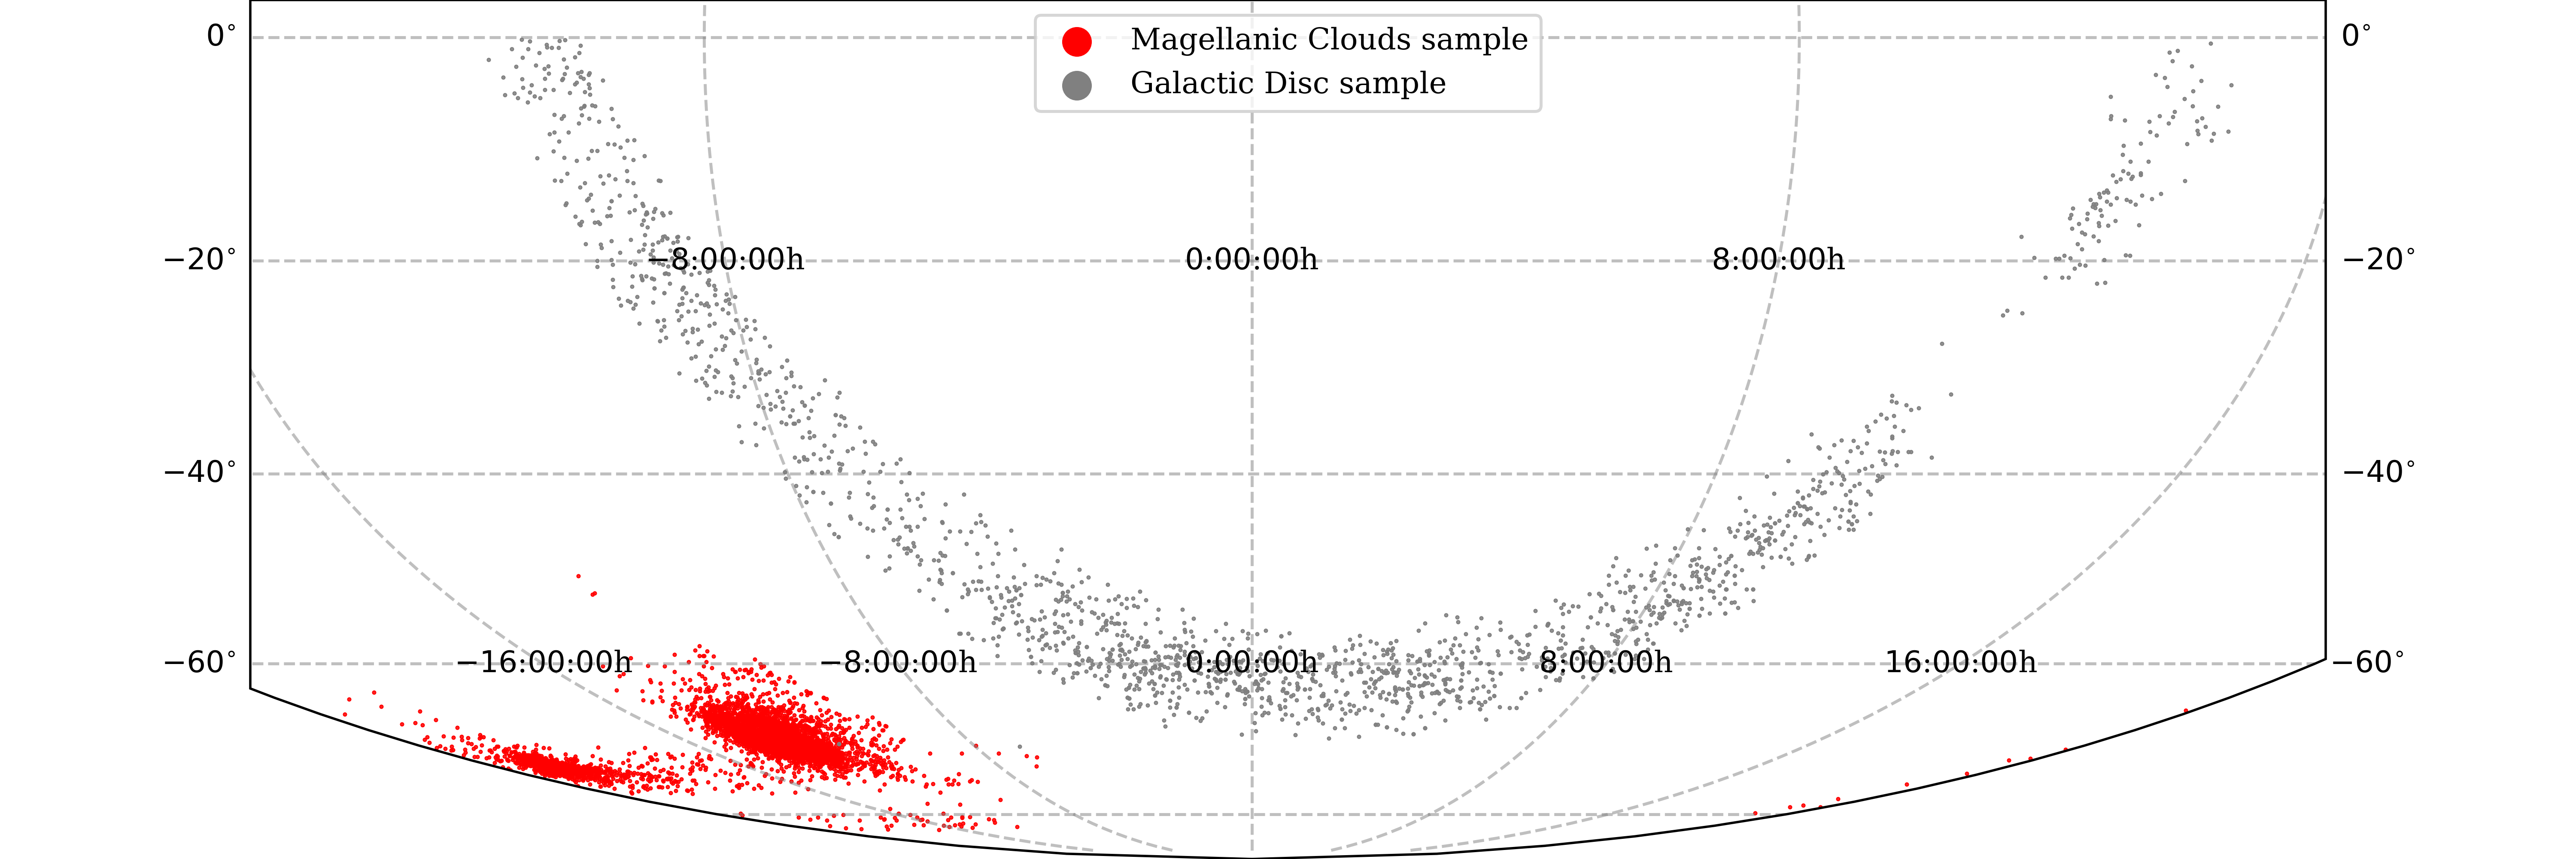
\includegraphics[scale=0.52]{plots/map_sample.png}
    \end{center}
    \caption{Distribution of objects in each sample.}
\end{figure}

\begin{figure}[H]
    \begin{center}
        \includegraphics[scale=0.6]{plots/HR_LMC_SMC.png}
    \end{center}
    \caption{HR diagram based on Gaia Data for objects that reside in Magellanic Cloud}
\end{figure}

\begin{figure}[H]
    \begin{center}
        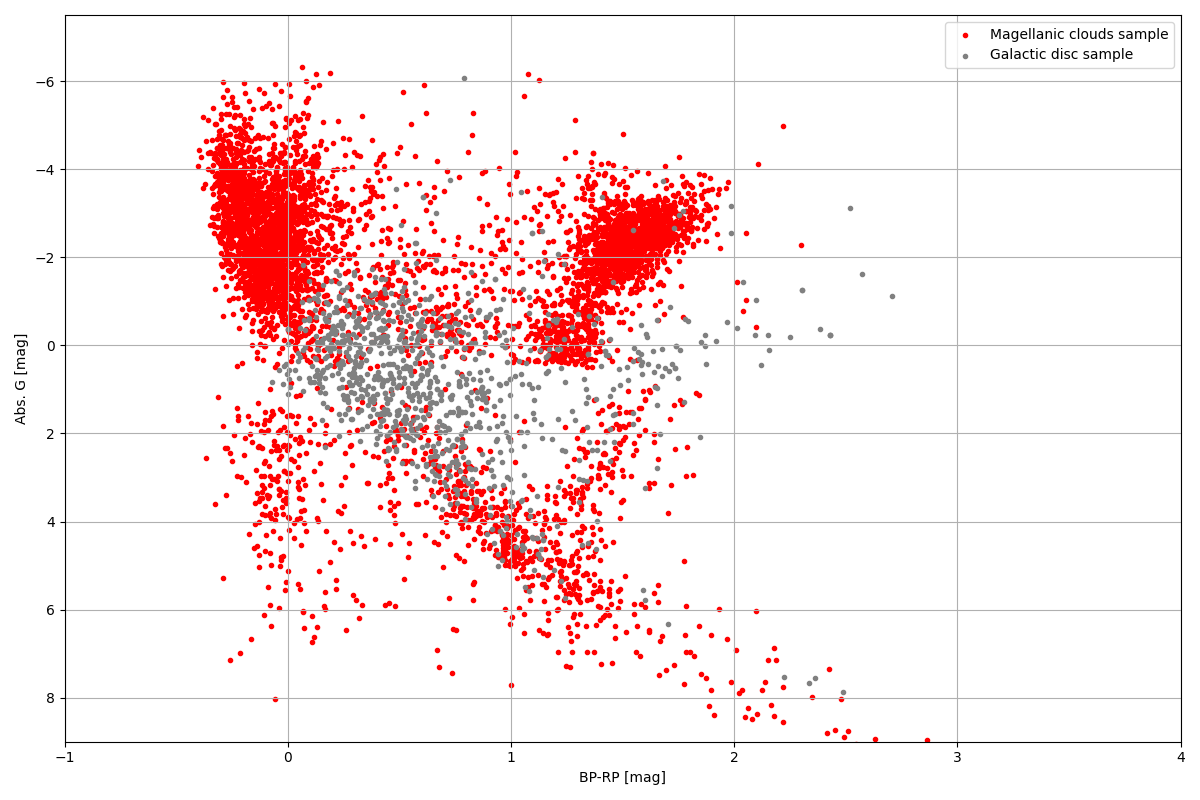
\includegraphics[scale=0.5]{plots/HR.png}
    \end{center}
    \caption{HR diagram based on Gaia Data for objects with measured parallax}
\end{figure}

Each object was analysed using ANOVA (analysis of variance) method \citep{schwarzenberg-czerny_advantage_1989} in order to determine period of light curve.
Then each light curve was fitted with $4$th degree harmonic model
\begin{equation}\label{harm}
    I(t)=A_0+\sum_i^4 A_{1i}\sin{\left(2\pi i\frac{t}{P}\right)}+A_{2i}\cos{\left(2\pi i\frac{t}{P}\right)}
\end{equation}
with sigma clipping threshold set at $3\sigma$ allowing to determine fourier coefficients from the relationship $A_i=\sqrt{A_{1i}^2+A_{2i}^2}$.
 Subsequently minimum mass ratio $q_{mmr}$ together with it's lower bound $\tilde{q}_{mmr}$ were calculated and previously described procedure of selecting candidates was carried out.
Objects with light curves indicating other type of variability then ellipsoidal one were removed together with those with period higher then
$50$ d. As we assume objects should be composed of star nearly filling Roche lobe suggesting rather small period. Exact value of threshold can be debated, here it's used as mean to 
remove pulsating stars that pollute our sample. After this part of preprocessing only $41$ objects from first sample left together with $22$ objects from second sample.
\begin{figure}
    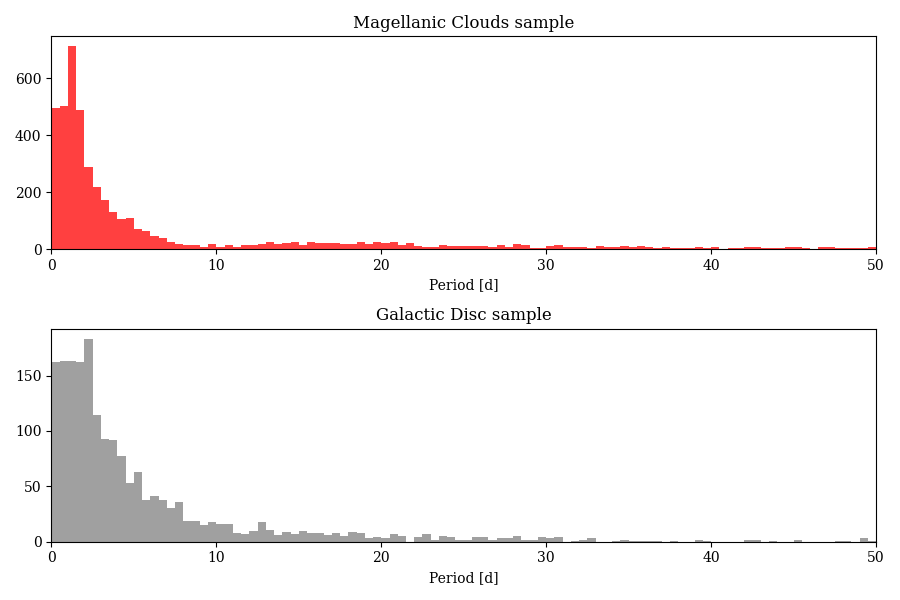
\includegraphics[scale=0.5]{plots/periods.png}
    \caption{Distribution of periods from the analysed samples.}
\end{figure}



\section{Spectral Energy Distribution}
Each object was cross matched  with Gaia DR3 catalogue obtaining parallax (denoted from here as $\pi_0$ together with uncertainty denoted as $\sigma_{\pi}$) estimates of objects. If parallax was statistically significant ($\pi>3\sigma_{\pi}$)
it was used to derive distance to object. For objects towards Magellanic Clouds many entries lacked statistically significant parallax indicating that they really reside in Magellanic Clouds
and do not line up accidentally.
In this case distance estimate $d_0$ and distance uncertainty $\sigma_d$ were based on the work \citep{jacyszyn-dobrzeniecka_ogle-ing_2016} assuming that presented distribution 
of cepheids reflects underlying distribution of stars in sample.
In the case of LMC and SMC assumed distance estimates were  $d_{LMC}=49.93\pm1.79$ kpc and  $d_{SMC}=64.62\pm4.95$ kpc respectively. 

To further investigate nature of objects spectral energy distribution analysis was 
performed with two models: single star model and double star model. Main goal of this type of analysis is to use photometry from various parts of spectra to
reconstruct whole spectral characteristic and hence obtain parameters of our object temperature.
Single star model depends on three free parameters: logarithm of temperature $\log_{10}T$ (measured in kelvins), logarithm of luminosity $\log_{10} L$ (measured in $L_{\odot}$) while third 
parameter was either parallax (if one was measured) or distance if it wasn't available. In the case of double star model there were two additional parameters describing 
second star $\log_{10} T_2$ and $\log_{10} L_2$. In the case of the first model star was assumed to be main sequence object (MS) with $\log{g}=4$. In double star model more massive star 
was assumed to have $\log{g_1}=4$ as in the first case while second object was assumed to be a giant with $\log{g_2}=2$. Objects with statistically significant parallax were assumed to have 
solar like metallicity ($Z=0.013$) as they reside inside galactic disc while objects in Magellanic Clouds 
were assumed to have metallicity equal to $Z=0.010$ in the case of LMC/MBR and $Z=0.005$ in the case of SMC.
BaSeL library of stellar spectra \citep{lejeune_standard_1998} was used to find spectrum for any given $\log_{10}{T}$, $\log_{10} L$, $d$ 
by means of interpolation as implemented in python library
\texttt{pystellibs}\footnote{https://github.com/mfouesneau/pystellibs}.
Theoretically calculated stellar spectrum is then processed using \texttt{pyphot}\footnote{https://github.com/mfouesneau/pyphot} 
Python library yielding observed magnitude in required filter.

In order to find set of best fitting parameters Bayesian approach was adopted. Let's denote set of observed magnitudes as $\tilde{m}_i$, theoretically predicted
magnitudes as $m_i$ while errors of magnitudes as $\sigma_i$. Let's denote $\mathcal{U}(a,b)$ to be uniform distribution with support in form of interval $[a,b]$ and $\mathcal{N}(\mu,\sigma^2)$ as
normal distribution with mean $\mu$ and variance $\sigma_i^2$. In order to prepare Bayesian model one need to specify probability distributions that allow to evaluate likelihood of 
data. Each of the observed magnitudes $\tilde{m}_i$ is expected to be normally distributed with mean $m_i$ and variance $\sigma_i^2$ while prior distributions on each of the three parameters
is either uniform in case of $\log_{10} T$ and $\log_{10} L$ or normal in case of distance or parallax. Detailed model can be written as:
\begin{align}
    \log_{10}{T}\sim \mathcal{U}(3.31,4.6)\\
    \log_{10}{L} \sim \mathcal{U}(-3,5)\\
    d \sim \mathcal{N}(d_0,\sigma_d^2) \textrm{ or } \\
    \pi \sim \mathcal{N} (\pi,\sigma_{\pi}^2)\\
    \tilde{m}_i\sim \mathcal{N}(m_i(\log_{10} T, \log_{10} L, d ),\sigma_i^2) \textrm{ or }\\
    \tilde{m}_i\sim \mathcal{N}(m_i(\log_{10} T, \log_{10} L, \pi ),\sigma_i^2)
\end{align}
where  $m_i(\log_{10} T, \log_{10} L, d )$ is written to indicate that predicted magnitude is function of parameters. 
Similarly we can write down our second model together with priors for parameters
\begin{align}
    \log_{10}{T_1}\sim \mathcal{U}(3.31,4.6)\\
    \log_{10}{L_1} \sim \mathcal{U}(-3,5)\\
    \log_{10}{T_2}\sim \mathcal{U}(3.444,4.21)\\
    \log_{10}{L_2} \sim \mathcal{U}(-3,5)\\
    d \sim \mathcal{N}(d_0,\sigma_d^2) \textrm{ or } \\
    \pi \sim \mathcal{N} (\pi,\sigma_{\pi}^2)\\
    \tilde{m}_i\sim \mathcal{N}(m_i,\sigma_i^2)
\end{align}
where we hidden explicit dependence of $m_i$ on parameters for clarity. In both cases normal distribution is truncated to positive numbers as we do 
not permit negative parallax/distance. Range on the logarithm of temperature is limited due to boundaries of library while limit of the logarithm of luminosity is 
set in the boundaries in order to eliminate possible unphysical solutions.
Under those assumptions log-likelihood function can be written as 
\begin{align}
    \mathcal{L}=-\sum_i\frac{(\tilde{m}_i-m_i)^2}{2\sigma_i^2}-\frac{(d-d_0)^2}{2\sigma_d^2} \textrm{ or }\\
    \mathcal{L}=-\sum_i\frac{(\tilde{m}_i-m_i)^2}{2\sigma_i^2}-\frac{(\pi-\pi_0)^2}{2\sigma_{\pi}^2}
\end{align} depending whether distance or parallax was used. 

Following catalogues were used to assemble SEDs:
\begin{enumerate}
\item Catalogues shared by both samples of objects:
\begin{itemize}
    \item 2MASS survey \citep{skrutskie_two_2006}
    \item Gaia DR2 \citep{gaia_collaboration_gaia_2018}
    \item VISTA Hemisphere Survey DR5 \citep{mcmahon_vizier_2021}
    \item ALLWISE/WISE survey (\citet*{wright_wide-field_2010} \citet*{cutri_vizier_2021})
    \item GALEX Survey \citep{bianchi_galex_2011}
    \item Spitzer IRAC data \citep{meixner_spitzer_2006}
    \item Denis survey  \citep{denis_vizier_2005}
    \item SkyMapper DR2 (\citet*{wolf_skymapper_2018}\citet*{onken_skymapper_2019})
    \item XMM Optical Monitor data \citep{page_xmm-newton_2012}
\end{itemize}
\item Catalogues exclusive to the Magellanic Clouds:
\begin{itemize}
    \item VISTA Magellanic Cloud survey DR4 \citep{cioni_vizier_2017}
    \item Denis cataloug of objects in Magellanic Clouds \citep{cioni_denis_2000}
    \item Magellanic Clouds Photometric Survey: SMC and LMC (\citet*{zaritsky_magellanic_2002} \citet*{zaritsky_magellanic_2004})
\end{itemize}
\item Catalogues exclusive to the Galactic Disc:
\begin{itemize}
    \item Bochum Galactic disc survey \citep{hackstein_bochum_2015}
    \item AAVSO Photometric All Sky Survey DR9 \citep{henden_apass_2015}
    \item VISTA Variable in Via Lactea Survey DR2 \citep{minniti_vizier_2017}
\end{itemize} 
\end{enumerate}. In the case of magellanic clouds extinction estimates were based on the map \citep{skowron_ogle-ing_2021} while in the case of Galactic disc extinction
was obtained using \texttt{mwdust} \citep{bovy_galactic_2016} Python library with 3D dust map beeing combination of \citep{green_3d_2019}, \citep{greiner_unusually_2001},
\citep{drimmel_three-dimensional_2003}. In the calculations Cardeli extinction law was assumed \citep{cardelli_relationship_1989}
and python implementation from \texttt{extinction}\footnote{https://extinction.readthedocs.io/en/latest/index.html} was used.
Using described setup MCMC python based library \texttt{emcee}\footnote{https://emcee.readthedocs.io/en/stable/} \citep{foreman-mackey_emcee_2013}
was used to construct compact library\footnote{https://github.com/Wesenheit/Iris} of routines used to sample from the posterior of our models allowing to estimates parameters together
with associated uncertainties. In order to help to decide between models 
BIC score was used 
\begin{equation}
    BIC=k\log{n}-2\mathcal{L}
\end{equation} where $k$ is number of estimated parameters and $n$ is  number of data points. From all objects $13$  were selected based on high quality fit with single star model while one of the objects was selected due to observed X-ray emission 
that can indicate existence of accretion disc. Complete list of objects together with key parameters is listed in table \ref{objects}.
\begin{table}[H]
    \scriptsize
    \centerline{
    \begin{tabular}{llllllllllll}
    Name&     Period [d]&     $q_{mmr}$ & $\tilde{q}_{mmr}$   &    RA [deg]        &  DEC [deg]        &   $A_0$    &      $A_1$ &   $A_2$     &    $A_3$     &     $A_4$  & $\pi_0$ [mas] \\
    BLG986.08.7     & $0.5132$  & $1.464$ & $1.029$  & $260.451241$ & $-43.019464$ & $12.192$ & $0.0028$  & $0.0985$ & $0.0039$  & $0.0093$ & $1.20$ \\
    GD2246.03.18414 & $0.4270$ & $2.299$ & $1.548$ & $179.327372$ & $-57.091968$ & $12.0764$ & $0.0045$  & $0.1090$ & $0.0030$ & $0.0106$  & $1.41$ \\
    GD1097.20.23000 & $0.4570$ & $9.739$ & $5.178$  & $252.108419$ & $-44.137004$ & $11.782$ & $0.0008$ & $0.1414$  & $0.0029$ & $0.0200$  &  $1.78$ \\
    GD1448.27.17    & $1.2410$  & $1.777$ & $1.233$ & $139.969949$ & $-45.759178$ & $11.875$ & $0.0115$  & $0.1035$ & $0.0030$  & $0.0056$  &  $0.77$ \\
    BLG931.27.36745 & $0.7050$   & $2.437$  & $1.628$ & $261.74489$  & $-40.31792$  & $11.633$ & $0.0033$ & $0.1113$ & $0.0026$ & $0.0105$ & $1.46$     \\
    GD1070.18.22288 & $45.1467$  & $7.409$ & $3.726$ & $257.007546$ & $-41.048747$ & $11.369$ & $0.0091$  & $0.1362$  & $0.0043$  & $0.0049$ &   $1.03$ \\
    LMC574.11.3407  & $0.2551$ & $1.479$ & $1.026$ & $80.1415$    & $-63.185667$ & $16.919$ & $0.0064$ & $0.0989$ & $0.0013$ & $0.0092$  &  $0.45$ \\
    LMC606.30.48    & $0.2698$   & $1.668$  & $1.113$ & $92.27575$   & $-63.376167$ & $15.906$ & $0.0141$  & $0.1019$ & $0.0038$  & $0.0122$ &   $0.52$ \\
    LMC751.15.2886  & $0.3753$ & $1.703$ & $1.161$  & $98.082958$  & $-66.307861$ & $16.958$    & $0.0090$  & $0.1024$ & $0.0012$ & $0.0121$  &  $0.18$ \\
    MBR108.18.3     & $0.2947$  & $1.487$ & $1.024$ & $33.257292$  & $-72.993167$ & $13.376$ & $0.0063$ & $0.0989$ & $0.0033$  & $0.0128$  &  $1.10$ \\
    MBR236.09.433   & $0.4398$  & $1.511$ & $1.070$ & $50.642958$  & $-80.540667$ & $14.585$ & $0.0024$ & $0.0994$  & $0.0028$ & $0.0089$  &  $0.47$ \\
    SMC711.22.1068  & $0.4466$  & $2.346$  & $1.555$ & $9.833875$   & $-70.378028$ & $13.226$ & $0.0029$  & $0.1104$ & $0.0053$  & $0.0154$ & $0.66$     \\
    SMC720.28.40576 & $0.5674$ & $4.290$  & $2.555$ & $11.938042$  & $-73.13625$  & $16.367$  & $0.0017$ & $0.1246$ & $0.0037$  & $0.0035$ &  $-$    \\
    SMC742.26.330   & $0.3453$ & $1.676$ & $1.118$ & $350.85925$  & $-77.530417$ & $13.864$ & $0.0042$   & $0.1020$ & $0.0049$ & $0.0074$ & $1.07$   
    \end{tabular}
    }
    \caption{Selected objects together with period, estimated mass ratios, coordinates, fourier coefficients ($A_i$) and parallax from Gaia DR3}\label{objects}
\end{table}
What should be emphasised here is meaning of BIC score. As we assume little about our objects especially we do not investigate best fitting 
$\log{g}$ which can be crucial to estimate stellar parameters. Due to this effect it's unreasonable to calculate values of $\chi^2$ and compare them 
across objects as few of them can be better fitted with given metallicity/$\log{g}$.
Single model SED fits together with light curves are presented in appendix.
\chapter{Results}
\section{Physical parameters of objects}
Each of $14$ final object was further investigated using available data in order to determine physical properties of objects.
Out of all $14$ objects $12$ of are of spectral types G or F, one object is of spectral type O while last one is composed of two objects. One of those objects is spectral type G while 
second is spectral type M. $13$ stars from the list have measured parallax from Gaia DR3 while one of the objects is located in SMC.
$11$ objects were selected based on good fit with single star model while one was selected due to counterpart emission i X-ray.

For each entry mass of object was estimated using PARSEC
(\citet*{costa_mixing_2019},\citet*{costa_multiple_2019}) evolutionary tracks. Assuming solar like metallicity simple approximate fits were obtained by choosing best fitting entry from PARSEC track using temperature and luminosity estimates from
SED fits.
\begin{table}[H]
    \normalsize
    \centerline{
    \centering
    \begin{tabular}{lllllll}
    Name& $T$ [K] & $R$ [$\textrm{R}_\odot$]&$E(B-V)$ & $d$ [kpc] & BIC & $M_{PARSEC}$ [$\textrm{M}_\odot$]\\
    BLG986.08.7     & $6118^{+19}_{-20}$ & $2.22\pm 0.01$ & $0.226$ & $0.83\pm 0.01$ & $193.3$ & $1.3$ \\
    GD2246.03.18414 & $7246\pm 41$ & $1.63\pm 0.02$ & $0.273$ & $0.71\pm 0.01$ & $91.4$ & $0.8$ \\
    GD1097.20.23000 & $6068\pm 13$ & $1.90\pm0.01$ & $0.221$  & $0.56\pm 0.008$ & $386$ & $1.2$ \\
    GD1448.27.17    & $8065\pm 39$ & $4.13\pm0.04$ & $0.611$  & $1.30\pm 0.02$ & $162.8$ & $2.3$ \\
    BLG931.27.36745 & $6434\pm 10$ & $2.25\pm0.01$ & $0.199$  & $0.69^{+0.04}_{-0.03}$ & $193.3$ & $1.4$ \\
    LMC574.11.3407  & $4680\pm 10$ & $1.01\pm0.01$ & $0.034$  & $2.20^{+0.46}_{-0.30}$ & $48.5$ & $-$ \\
    LMC606.30.48    & $5280\pm 11$ & $1.08\pm0.01$ & $0.047$  & $1.93^{+0.15}_{-0.12}$ & $101.7$ & $0.8$ \\
    LMC751.15.2886  & $5768\pm 6$ & $1.30\pm0.01$ & $-$  & $0.91\pm 0.01$ & $3318.9$ & $3.2$ \\
    MBR108.18.3     & $5943^{+23}_{-20}$ & $1.56\pm0.01$ & $0.000$  & $5.70^{2.98}_{-1.49}$ & $75.1$ & $1.1$ \\
    MBR236.09.433   & $6285\pm 8$ & $1.88\pm0.01$ & $-$  & $2.12\pm 0.07$ & $950.5$ & $1.2$ \\
    SMC711.22.1068  & $6717\pm 13$ & $1.99\pm0.01$ & $0.021$  & $1.52\pm 0.03$ & $1541.2$ & $1.4$ \\
    SMC720.28.40576 & $34183^{+985}_{-655}$ & $4.41^{+0.17}_{-0.24}$ & $0.095$  & $-$ & $263.7$ & $16$ \\
    SMC742.26.330   & $5615\pm 5$ & $1.57\pm0.01$ & $-$  & $0.93\pm0.01$ & $4736.4$ & $1$ \\  
    \end{tabular}
    }
    \caption{Estimated physical parameters of objects using single star model together with PARSEC mass estimates and extinction estimates.}\label{objects}
\end{table}

\section{Radial velocity semi-amplitude estimation from Gaia DR3 data}
Half of the objects from final list have available high-quality radial velocity information that is normally available for bright stars from Gaia DR3 catalogue. While estimate of radial velocity 
is based on median of observed radial velocity, error of this estimate is based on the epoch standard deviation of observed values. According to \citep{katz_gaia_2022} radial velocity error $\delta v$ 
is calculated via equation
\begin{align}
    \delta v=\sqrt{\sigma_{med}^2+0.11^2}\\
    \sigma_{med}=\sqrt{\frac{\pi}{2}}\frac{\sigma(V_j)}{\sqrt{N}}
\end{align}
where $\sigma(V_j)$ is standard deviation of radial velocity while $N$ stands for number of transits used to compute radial velocity. This simple formula allows to obtain variance of 
radial velocity measurements as 
\begin{equation}
    \sigma^2=\frac{2N}{\pi}\left((\delta v)^2-0.11^2\right)
\end{equation}
. It can be proven (for details see appendix A) that if we assume error is dominated by sinusoidal radial movement with amplitude $K$ 
variance of velocity will be equal to
\begin{equation}
    \sigma^2=\frac{K^2}{2}
\end{equation}.
Using this fact one can estimate semi-amplitude of velocity using Gaia measurements (that will be denoted from here as $K_{Gaia}$) as 
\begin{equation}
    K_{Gaia}=\sqrt{\sigma^2}\sqrt{2}=2\sqrt{\frac{N}{\pi}\left((\delta v)^2-0.11^2\right)}
\end{equation}
This radial velocity amplitude then is used to calculate binary mass function for each of objects using definition 
\begin{equation}\label{mass}
    f(M_1,M_2,i)=\frac{M_2^3 \sin{i}^3}{(M_1+M_2)^2}=\frac{K^3 P}{2\pi G}
\end{equation}
where $P$ stands for period while $G$ is gravitational constant. For each object with RV estimates based on aforementioned method mass functions were obtained and together with
information about radial velocity estimates are presented in table \ref{mass_function_table}.
For each object with PARSEC mass estimate lower boundary of companions mass was calculated by solving equation \ref{mass}
with  $\sin{(i)}=1$. Each of minimum masses were then plotted versus period of binary and are presented on \ref{lower_mass}
and placed into table as $M_{min}$.

In \citep{katz_gaia_2022} criterion was presented allowing to test whether radial velocity indicates variability based on values of {\it{rv\_chisq\_pvalue}}
and {\it{rv\_renormalised\_gof}}. Criterion states that objects with $N>10$, $T_{eff}\in [3900,8000]$ K, {\it{rv\_chisq\_pvalue}}$<0.01$ 
and {\it{rv\_renormalised\_gof}}$>4$ can be safely considered to be variable in radial velocity. Each object was tested using described method 
and results are presented in the table (in case of not enough data objects were labeled as unsure).
\begin{table}[H]
    \footnotesize
    \centering
    %\def\arraystretch{1.5}
    \setlength{\tabcolsep}{3pt}
    \begin{center}
    \begin{tabular}{lllllllll}
    Name & Period [d]& $RV$ [km/s]& $N$  &  $\delta v$  [km/s]   & $K_{Gaia}$ [km/s]  & $f(M_1,M_2,i)$ [M$_{\odot}$]& $M_{min}$ [M$_{\odot}$]&Variable RV?\\
%    GD1549.19.348   & $2.8224$   & $36.72$ & $21$ & $8.64$  & $44.67$   & $0.026$ &\\
    GD2246.03.18414 & $0.4270$ & $27.68$ & $25$ & $23.03$ & $129.93$ & $0.097$  & $0.80$ & Yes\\
    GD1097.20.23000 & $0.4570$ & $36.5$  & $10$ & $21.03$ & $75.03$  & $0.020$  & $0.37$& Unsure\\
    BLG986.08.7     & $0.5132$  & $-1.69$ & $15$ & $18.11$ & $79.14$   & $0.026$  & $0.43$& Yes\\
    BLG931.27.36745 & $0.7050$   & $-4.35$ & $8$  & $14.81$ & $47.26$  & $0.0077$ & $0.28$& Unsure\\
    GD1448.27.17    & $1.2410$  & $33.08$ & $22$ & $7.69$  & $40.69$  & $0.0086$ & $0.40$& Yes\\
    GD1070.18.22288 & $45.1467$  & $38.71$ & $20$ & $7.66$  & $38.65$  & $0.27$  & -- & Yes\\
    \end{tabular}
    \end{center}
    
    \caption{Estimated mass function using Gaia radial velocity error.}\label{mass_function_table}
\end{table}
\begin{figure}
    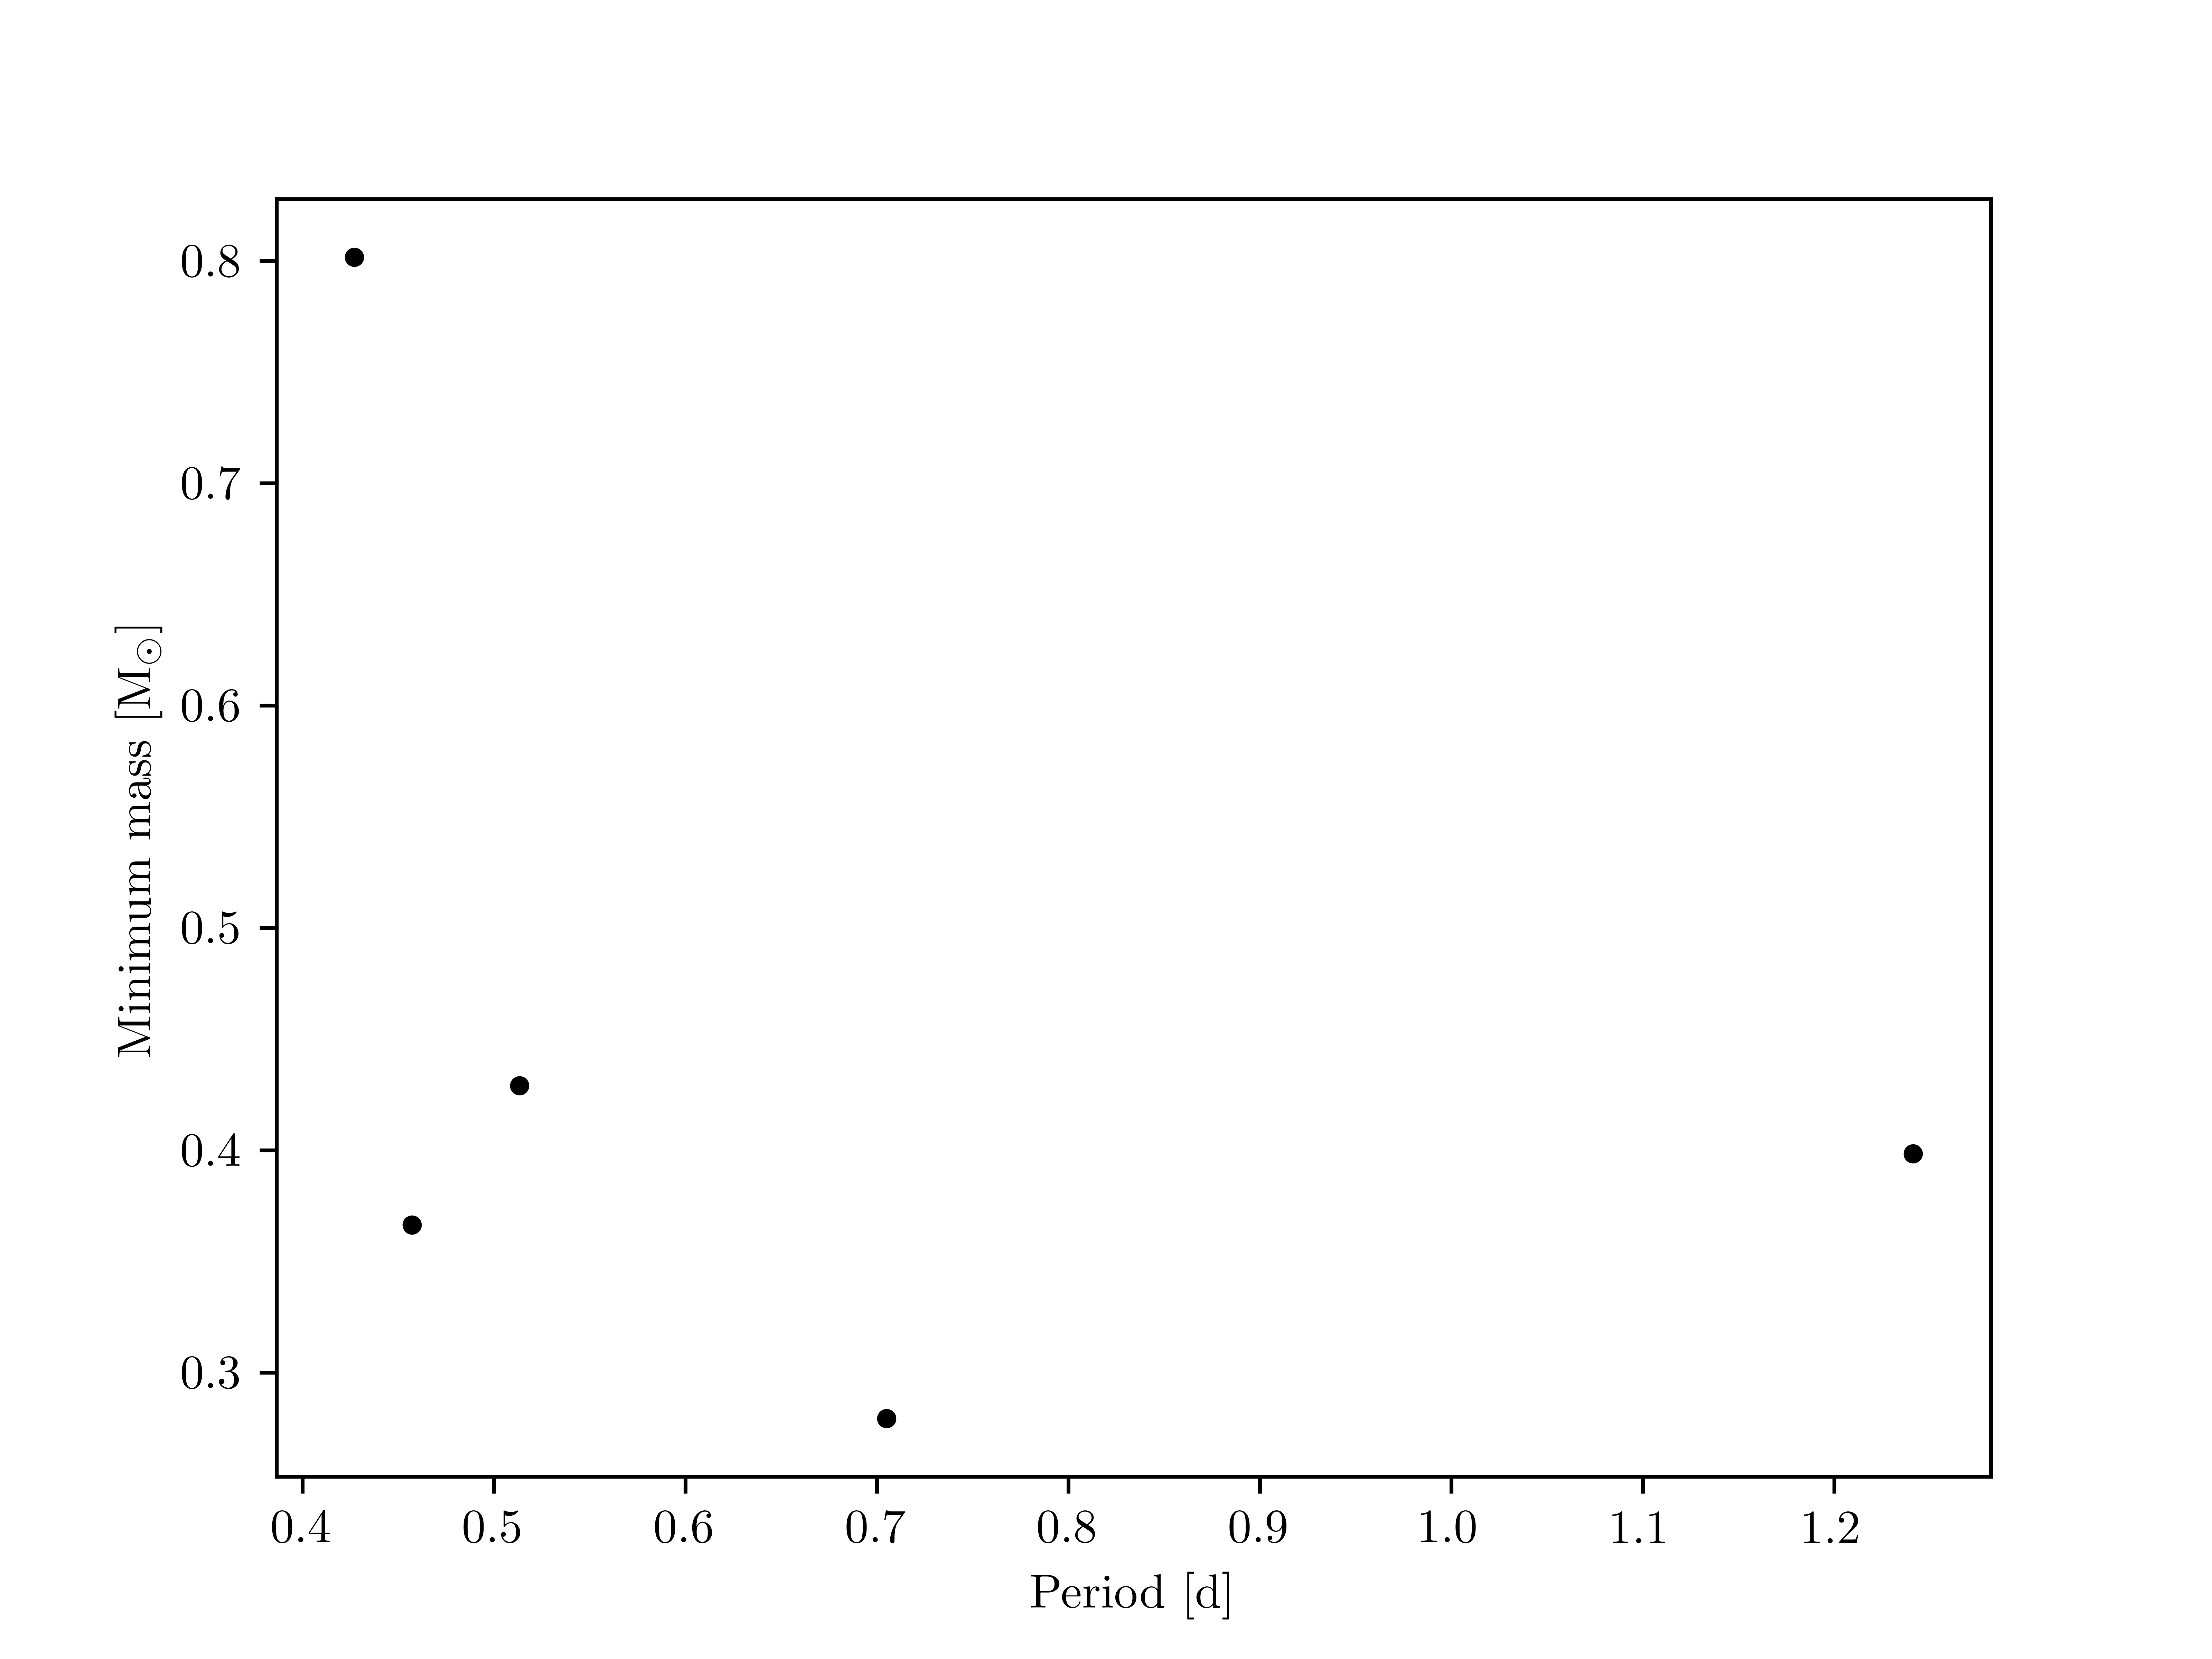
\includegraphics{plots/mass_minimum_estimate.png}
    \caption{Lower bound of companions mass.}\label{lower_mass}
\end{figure}

\section{Detailed analysis of objects}
In this section detailed characteristic of individual objects will be provided. It will be divided into $3$ subsections where first two will quickly cover information available for 
objects GD1070.18.22288 and GD1070.18.22288 while third one will be dedicated to rest.
\subsection{GD1070.18.22288}
GD1070.18.22280 has longest period from selected objects with $P\approx 45$ d and was listed as plausible candidate only due to the reported X-ray emission. Due to excess amount of observations in 
many parts of spectra it was possible to obtain high quality spectral energy distribution fit that revealed two sources with different temperatures, presented distribution can be 
seen on plot \ref{GD1070SED}.
\begin{figure}[H]
    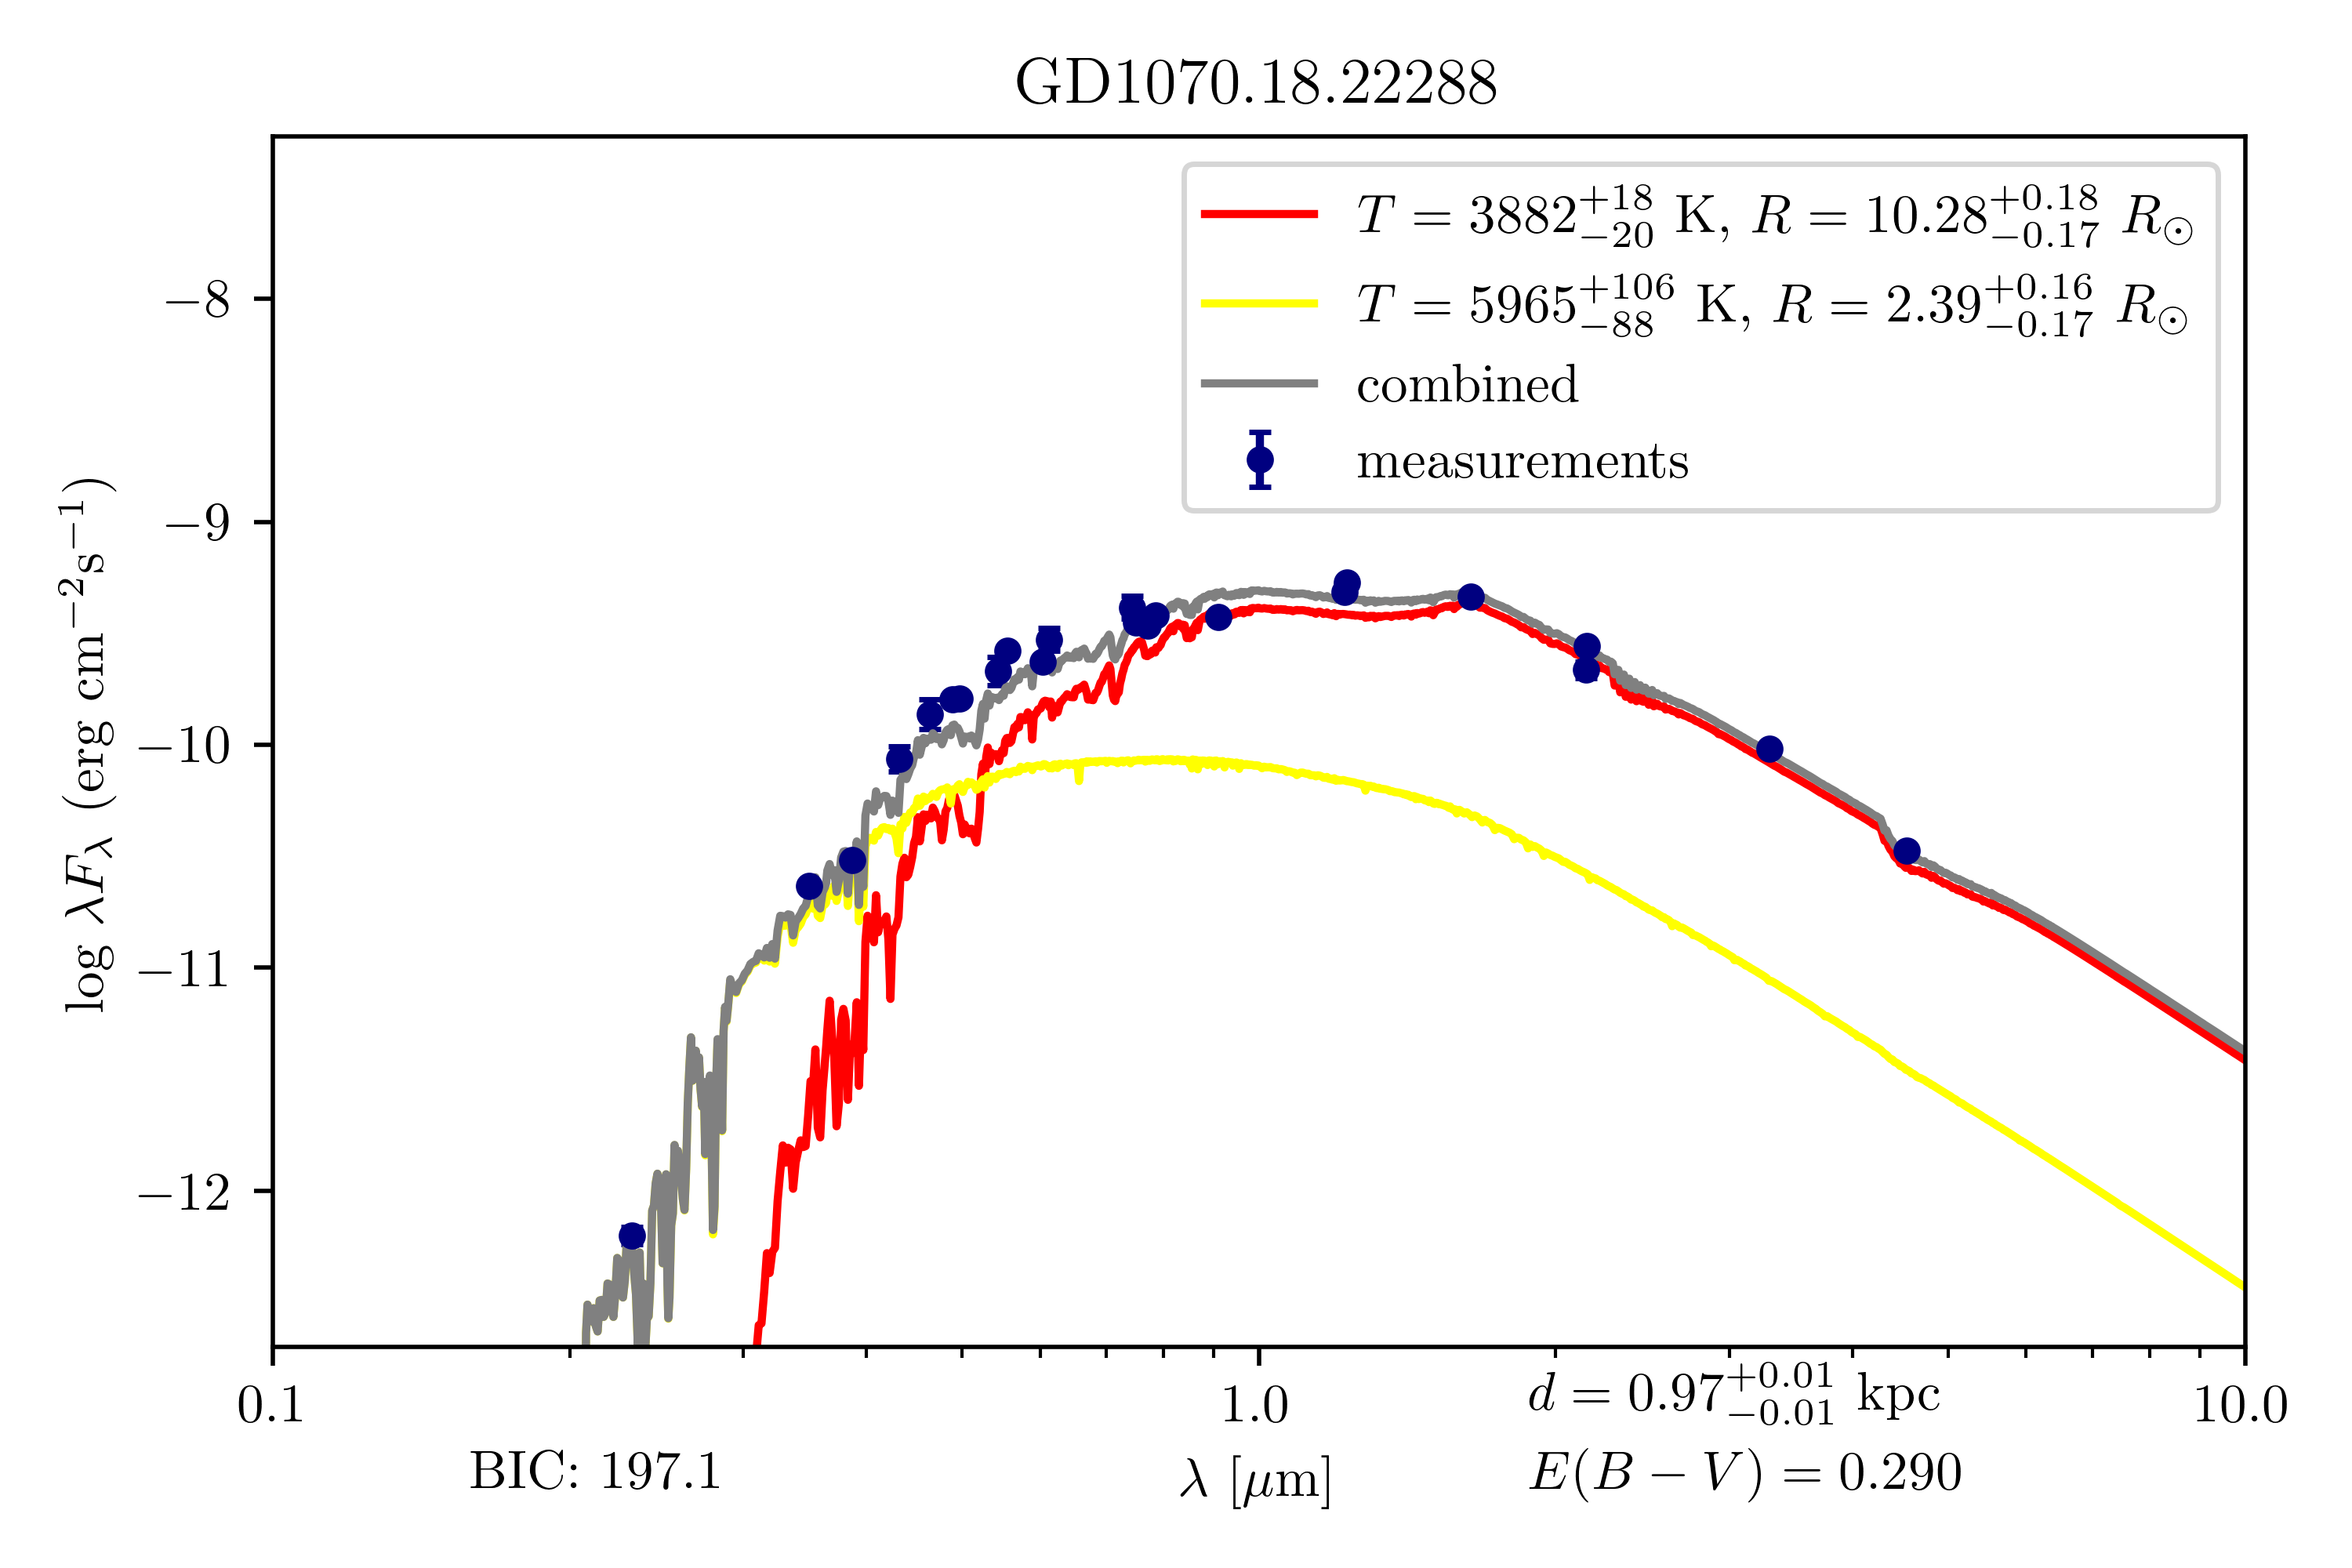
\includegraphics{plots/GD1070.18.22288/GD1070.18.22288_double_emcee.png}
    \caption{Spectral Energy Distribution fit for GD1070.18.22280 using model with two components.}\label{GD1070SED}
\end{figure}

One of the objects with rather low temperature of 
$T\approx 3800$ K has radius $R\approx 10$ $\textrm{M}_{\odot}$ and was quite distant from any evolutionary track in PARSEC database as it's probably giant stripped by 
it's companion. Object can be also found in ASAS-SN database \citep{jayasinghe_asas-sn_2019} under id J170801.81-410255.6 where it's classified as rotational variable star
with half of the period found in this work. It was observed by ASAS-SN in $V$ and SDSS $g$ band allowing to compare light curves with OGLE. Moreover 
it was observed in SDSS $i$ band by Bochum Disc Survey \citep{hackstein_bochum_2015}. Comparison between all light curves can be found on the plot \ref{comp}
\begin{figure}[H]
    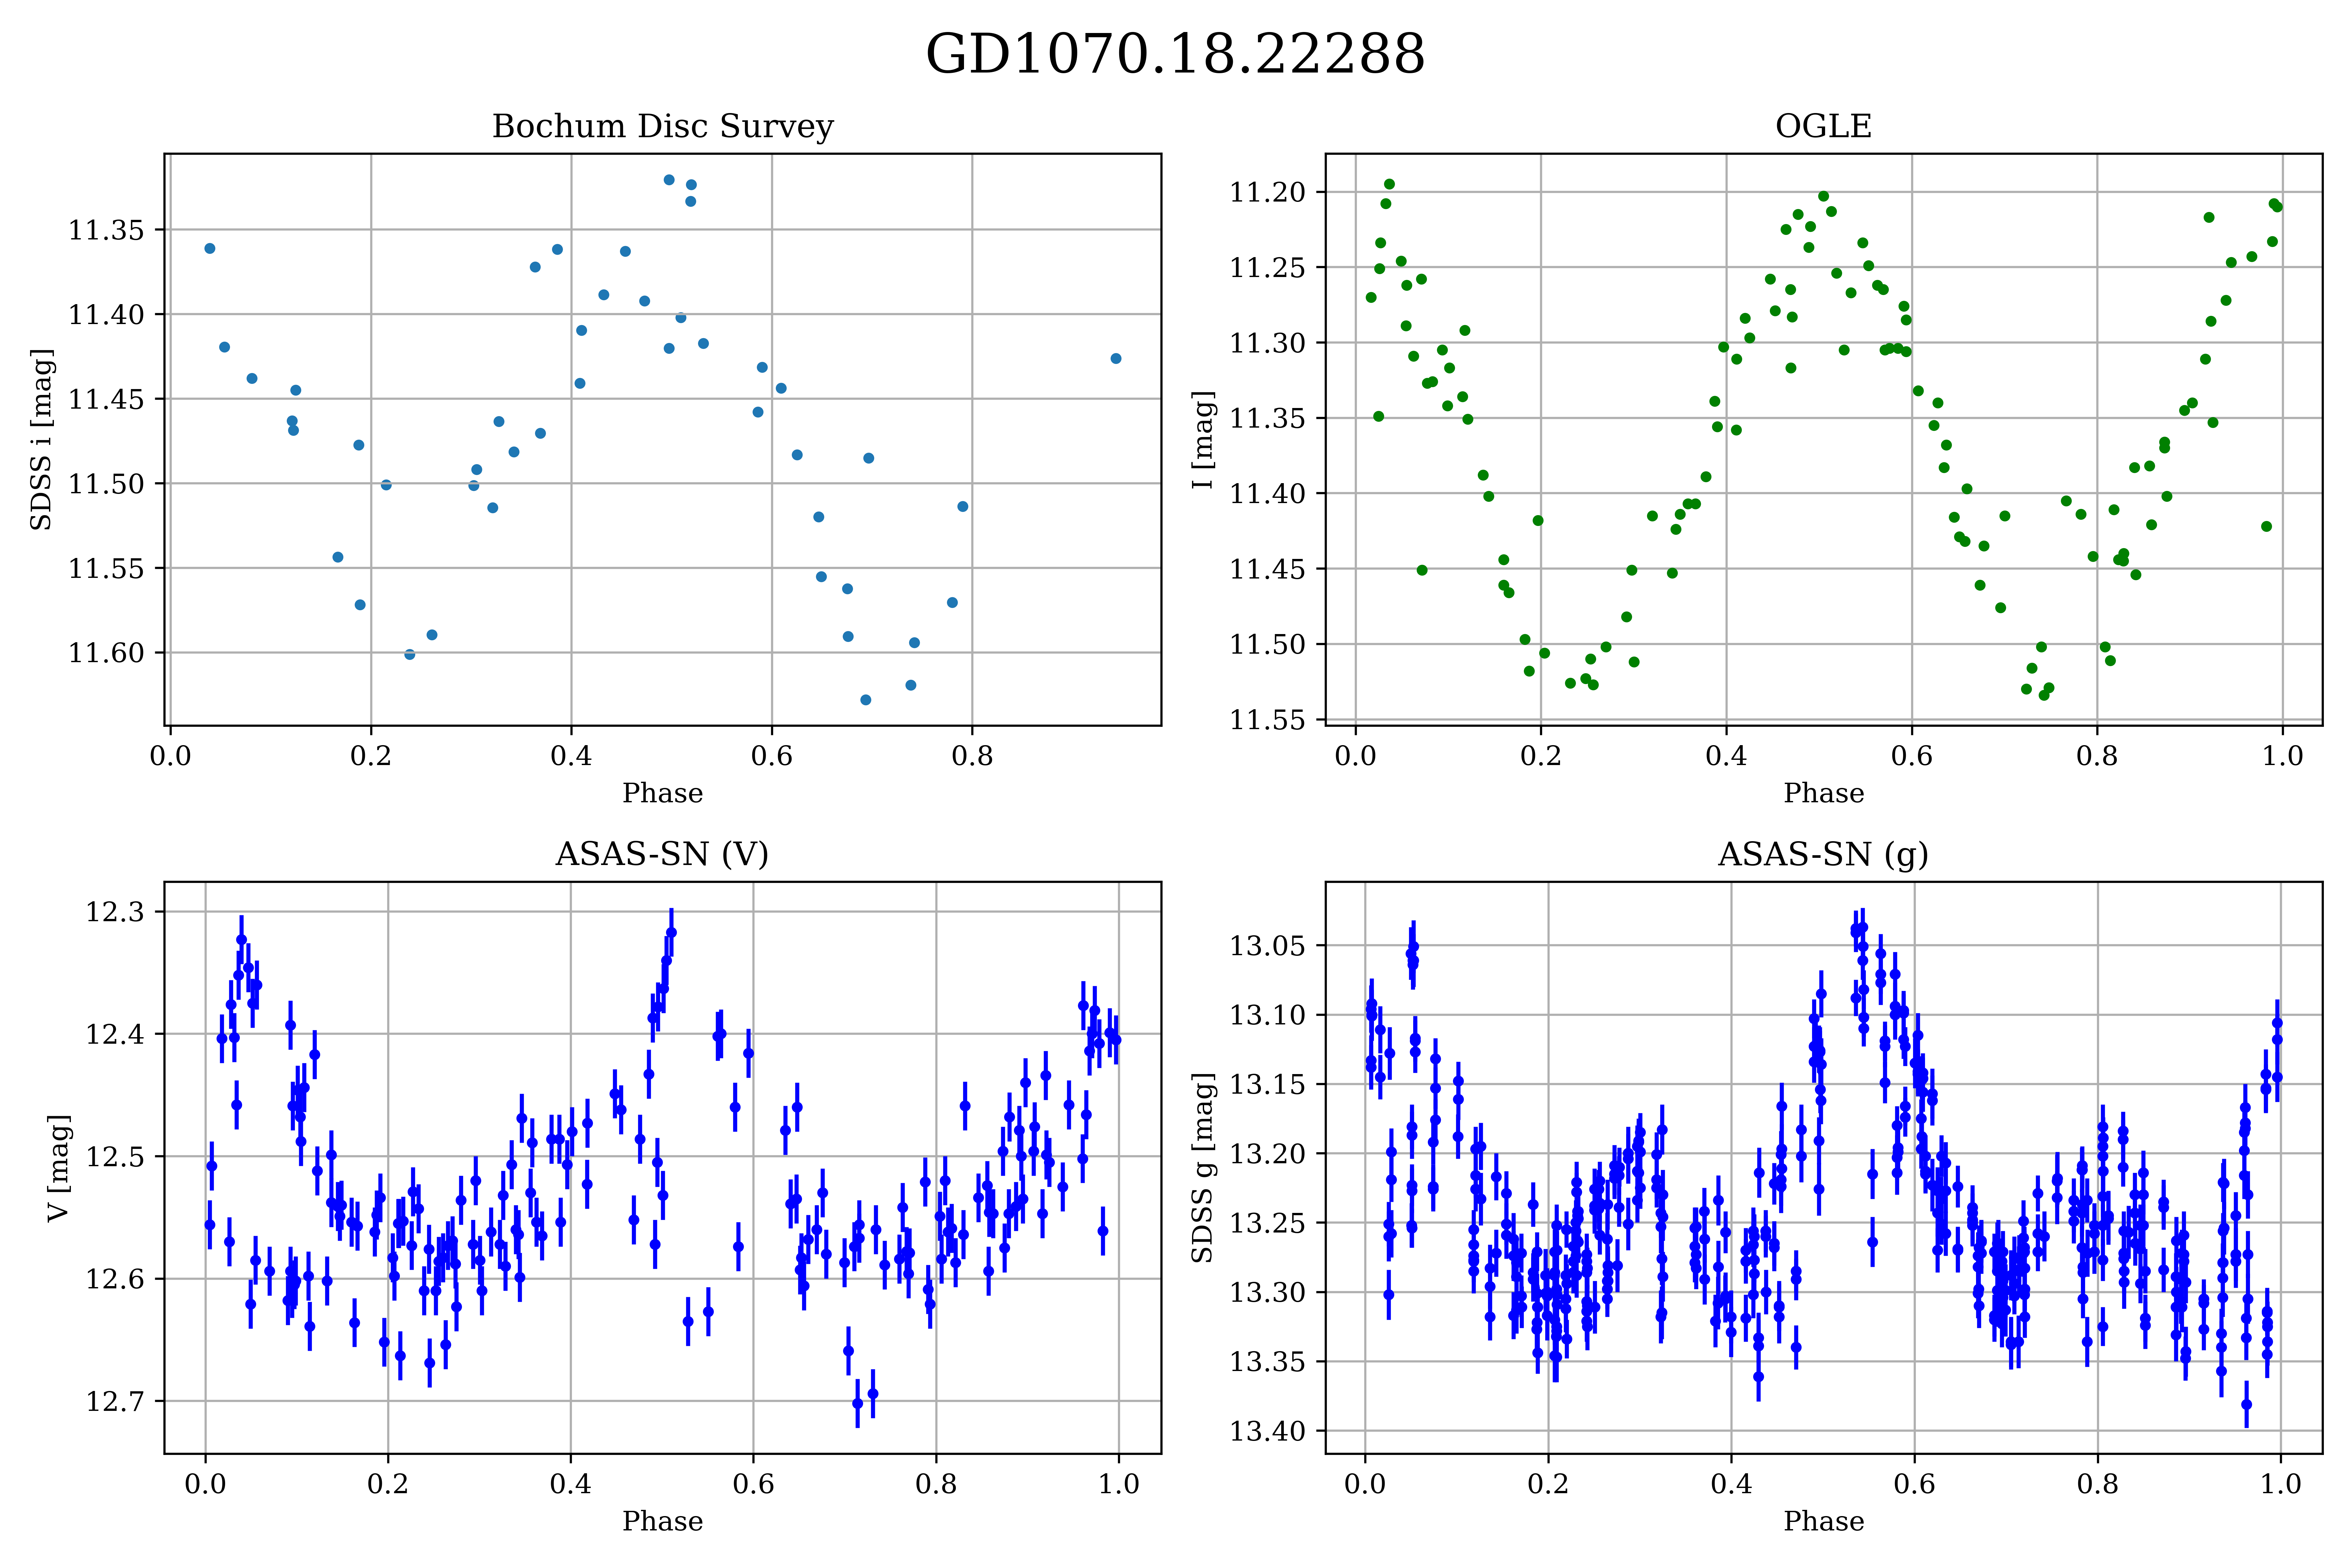
\includegraphics[scale=0.5]{plots/GD1070.18.22288/lc_comparsion.png}
    \caption{Light curves of GD1070.18.2288 in $4$ different bands}\label{comp}
\end{figure}
ASAS observation in g band can be traced back to 2016 and allow to get better insight into evolution of light curve over time, change of observed brightness is presented on the
plot \ref{evolution}. Object have also greatest value of mass function from whole sample that is equal to $\sim 0.25 \textrm{M}_{\odot}$. 

\begin{figure}[H]
    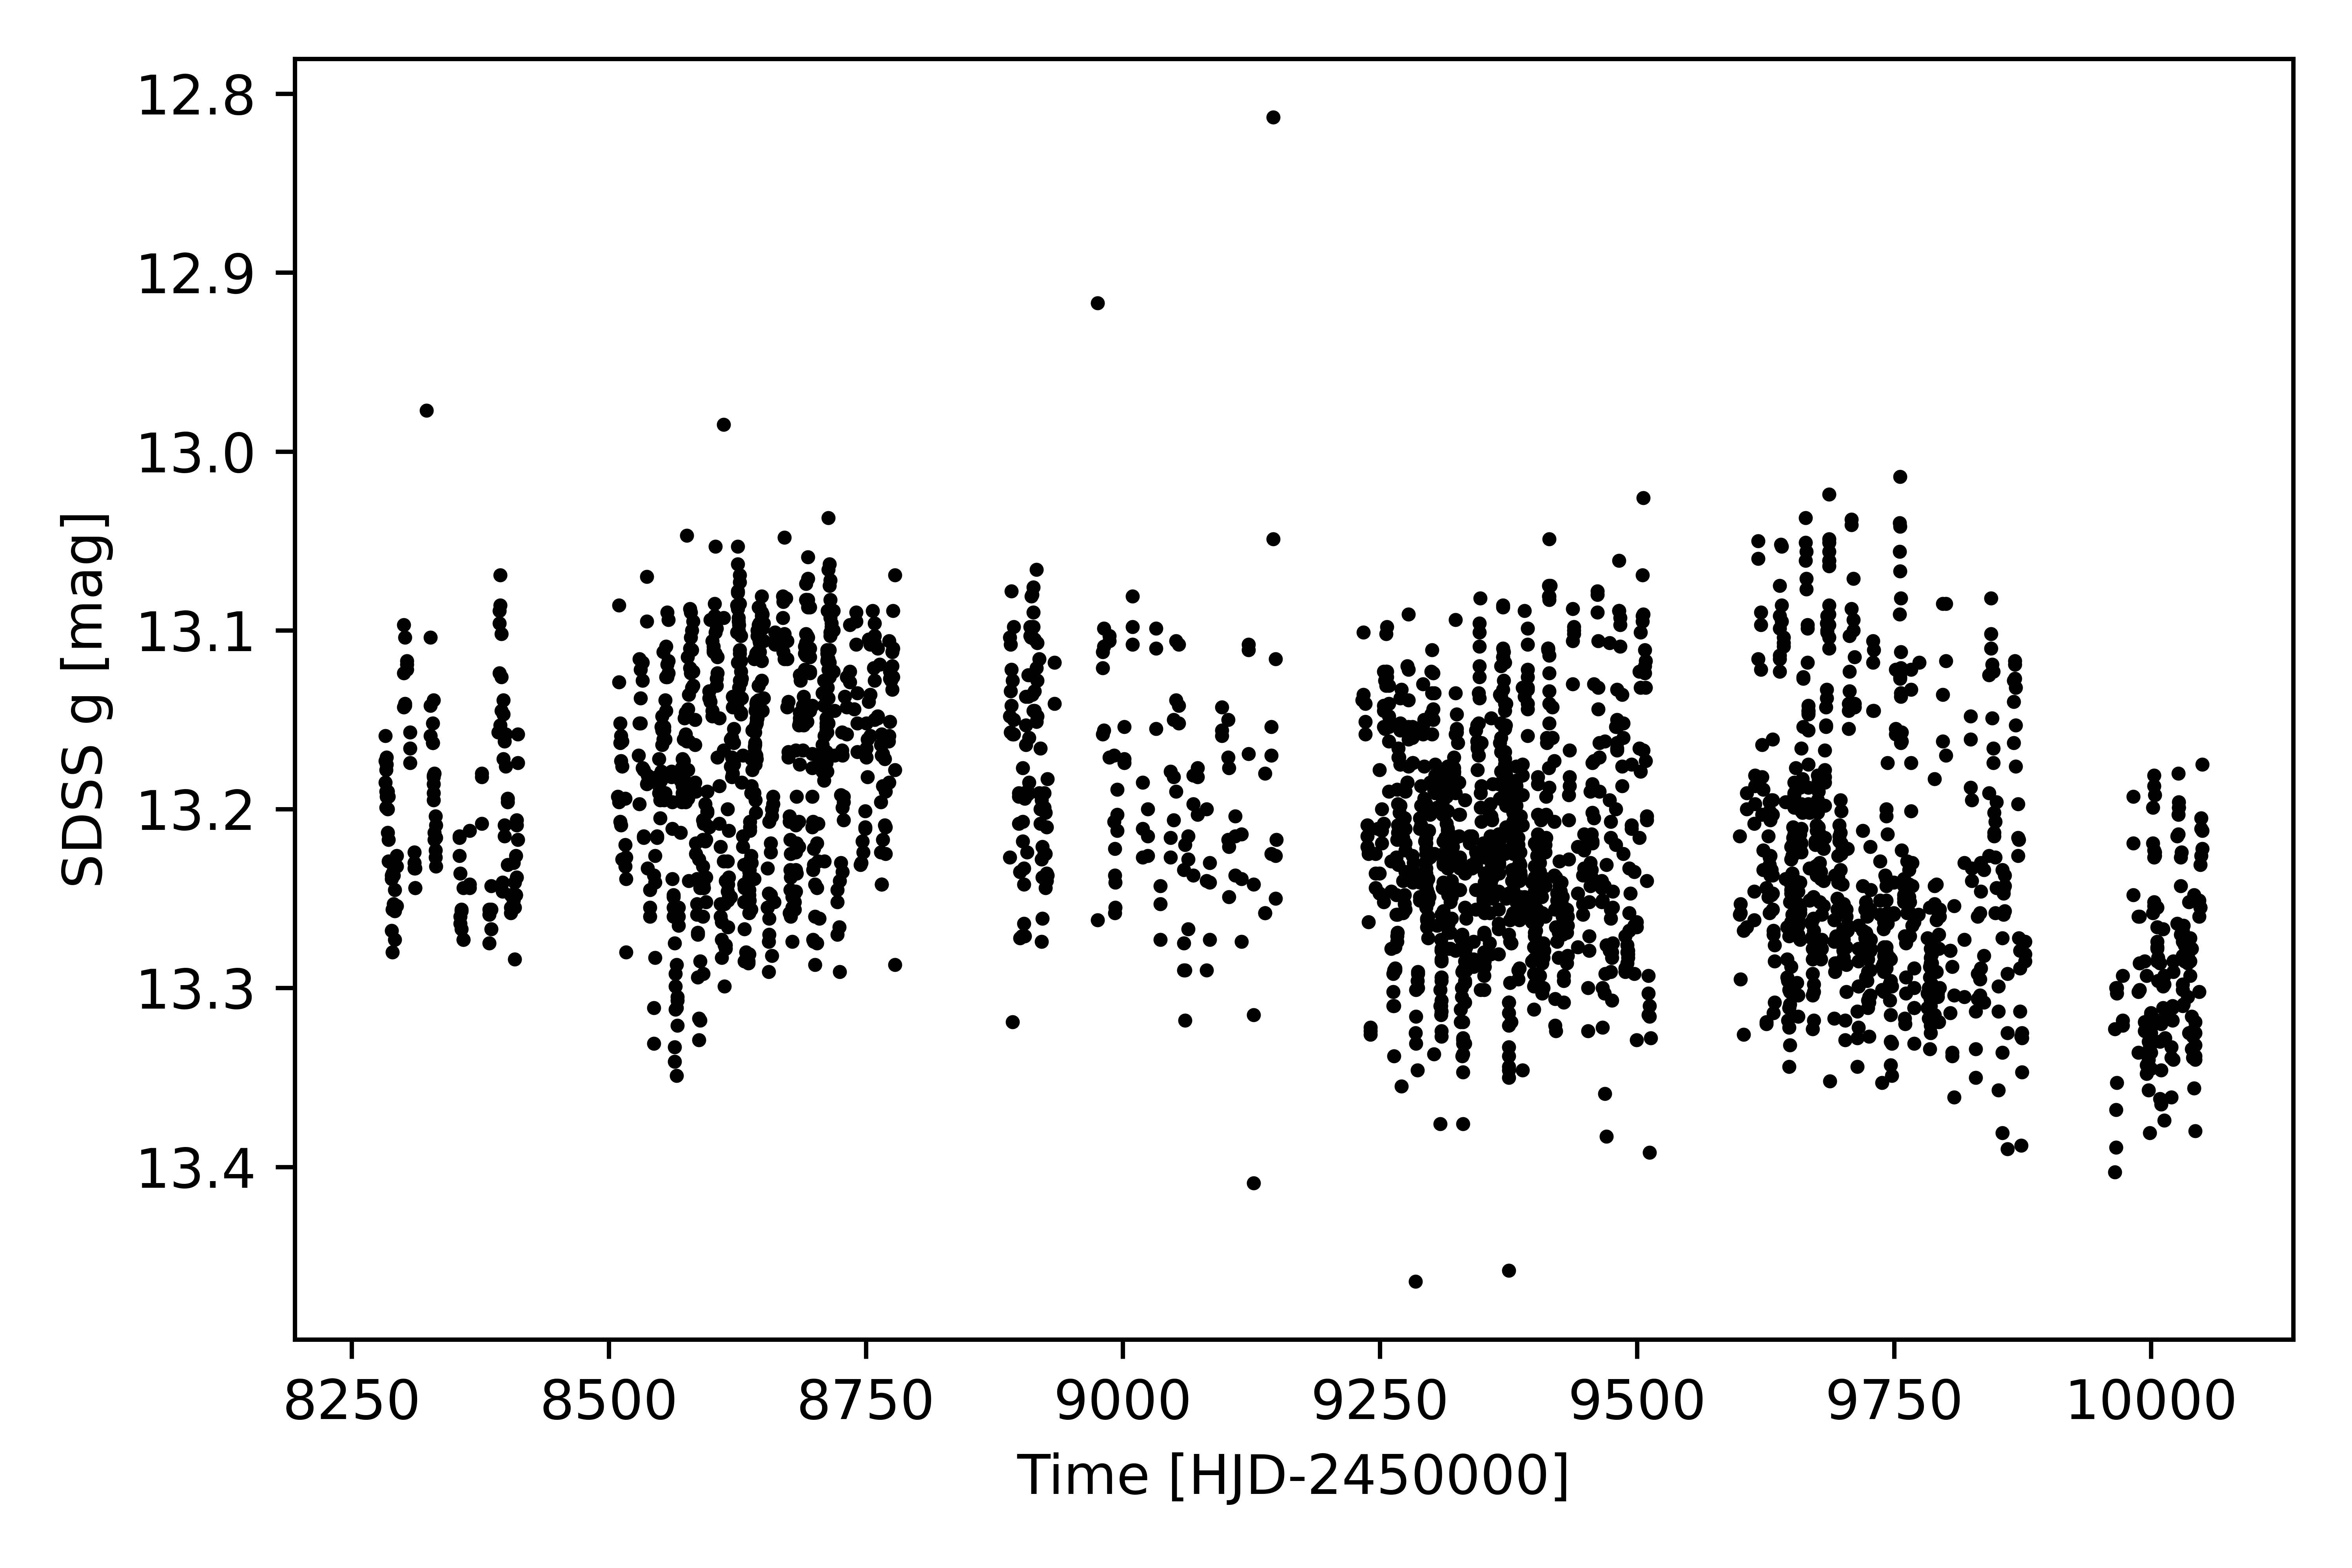
\includegraphics{plots/GD1070.18.22288/visibility_over_time.png}
    \caption{Change of brightness in SDSS g band over time  }\label{evolution}
\end{figure}

Object was observed in X-ray by Swift and XMM missions and published in serendipitous sources catalogs (\citep{evans_2sxps_2020} and \citep{traulsen_xmm-newton_2020}) with id names J170801.8-410254 and J170801.8-410255
respectively. Angular distance between position reported by XMM DR11 catalogs \citep{traulsen_xmm-newton_2020}  and OGLE position is $105$ mas and has reported statistical/positional error of order $365$ mas.
XMM object also came to attention 
due to gamma ray source source HESS J1708-410 \citep{aharonian_hess_2008} located $4.212$ arcminutes from estimated source position. Results from elongated 2-D Gaussian model fit to gamma 
excess yielded standard deviations $3.6$ arcminutes and $4.8$ arcminutes along principal axis. Up to date no plausible explanation was found to the origin
of aforementioned source despite multiple efforts and search in various parts of optical spectra. One particular work \citep{van_etten_multi-wavelength_2009} observed close neighbourhood of
gamma ray source and found emission from point source labeled in the publication as nr $1$ (hereinafter referred to as [VFH2009] 1).
This particular point source although quite faint coincides with  position of GD1070.18.22280 with accuracy of $382$ mas. 
In the publication it was found that X-ray emission is best fitted with absorbed power law by hydrogen density $n_H=2.0\times 10^{21}$ $\textrm{cm}^{-2}$.
No conclusion was reached although publication explored few possibilities of the potential origin of gamma emission including Pulsar Wind Nebulae kind scenario. Interestingly assumed 
distance of $3$ kpc based on radio observations is nearly $3$ times higher then one obtained using parallax from Gaia DR3. If emission really originates from the system 
based on the Gaia parallax luminosity in X band would be around $L_{X}=1.32\cdot10^{31}$ erg/s. 

As one can see on figure \ref{comp} there is discrepancy between curves in $I$ band and curves from ASAS-SN. This is due to the different time light curves were collected. OGLE 
light curve is composed from observations collected from $2456467$ to $2458734$ HJD but most samples were collected before $2457201$ HJD. On the other hand
observations from ASAS in $g$ band were collected after $2459797$ HJD. Using archival data from ASAS there is visible point around $2459100$ when period of the 
variable changes from $\sim 45$ d to nearly half the value around $\sim22.4$ d. This observation together with evolution of amplitude of the variability as presented on the
plot \ref{evolution} clearly suggest that object represents class of rotational variables. This can be also partially supported by the X ray emission from the system, 
it's widely known that many rotational variables like RS Canum Venaticorum can emit X rays with luminosity around $\sim 10^{31}$ erg/s  \citep{walter_x-rays_1980} so value obtained from XMM 
is consisted with emission from this type of system. It's hard to determine if OGLE curve exhibit similar changes in brightness as observations cover only relatively short period of time.
It's highly unlikely that variability in $I$ band is caused by ellipsoidal modulation if period would be equal to $45$ d as inferred radii are to small for the system to fill their Roche Lobes 
(unless system would have very small total mas). After investing all of the observational data it's hard to pinpoint true nature of the system. Most plausible 
explanation states that the system is similar to RS Canum Venaticorum variable which underwent mass transfer in the past. Colder star is covered in spots 
that emerge due to high magnetic fields, such stars can develop powerful coronal heating responsible for X-ray emission. Although one could investigate spectrum 
of object to find whether it's consisted with emission from hot plasma but as the object isn't ellipsoidal variable this line of investigation is dropped as it's beyond
scope of the work.% Despite lack of ellipsoidal modulation object may be interesting as it may still have greatest mass function.

\subsection{SMC720.28.40576}
\begin{figure}[H]
      \centering
      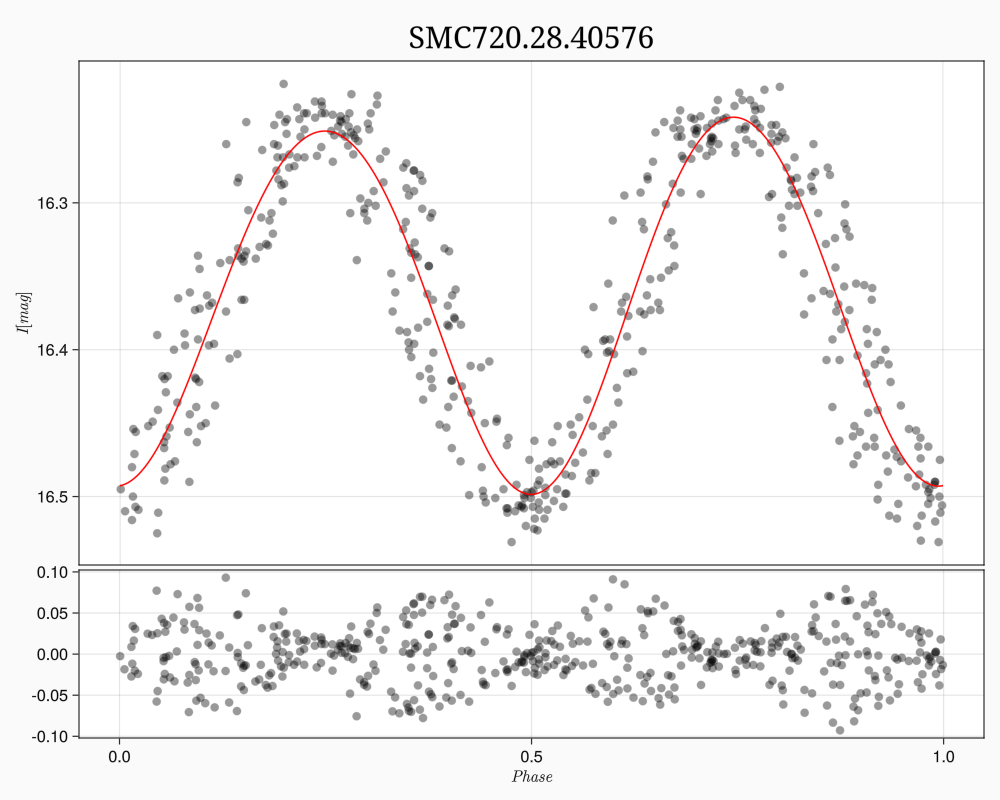
\includegraphics[scale=0.35]{plots/SMC720.28.40576_phase.png}
      \caption{Light curve of SMC720.28.40576 collected by project OGLE.}
      \label{SMC720:lc}
\end{figure}
SMC720.28.40576 is the only object in the sample that reside in Magellanic Clouds. It's very luminous and hot, 
estimated parameters suggest it's blue giant with spectral type O according to single model SED fit \ref{SMC720:sed}.
Estimated period of the variable is nearly half of day, such short period paired together with such high mass suggest very compact setup of stars.
PARSEC evolutionary tracks estimate mass of object around $16$  $\textrm{M}_{\odot}$. Star was published already by \citep{pawlak_ogle_2016} and classified as contact binary. Although
no companion is visible in SED distribution it might hide itself in the light of primary star.
No WISE source could be found as nearest detection is nearly $10$ arcsec away from the position, lack of any observations 
in W3 and W4 bands is very problematic as they allow to probe object in low temperatures.
No radial velocity from Gaia is available so mass function estimate remains unknown.
\begin{figure}[H]
    \centering
    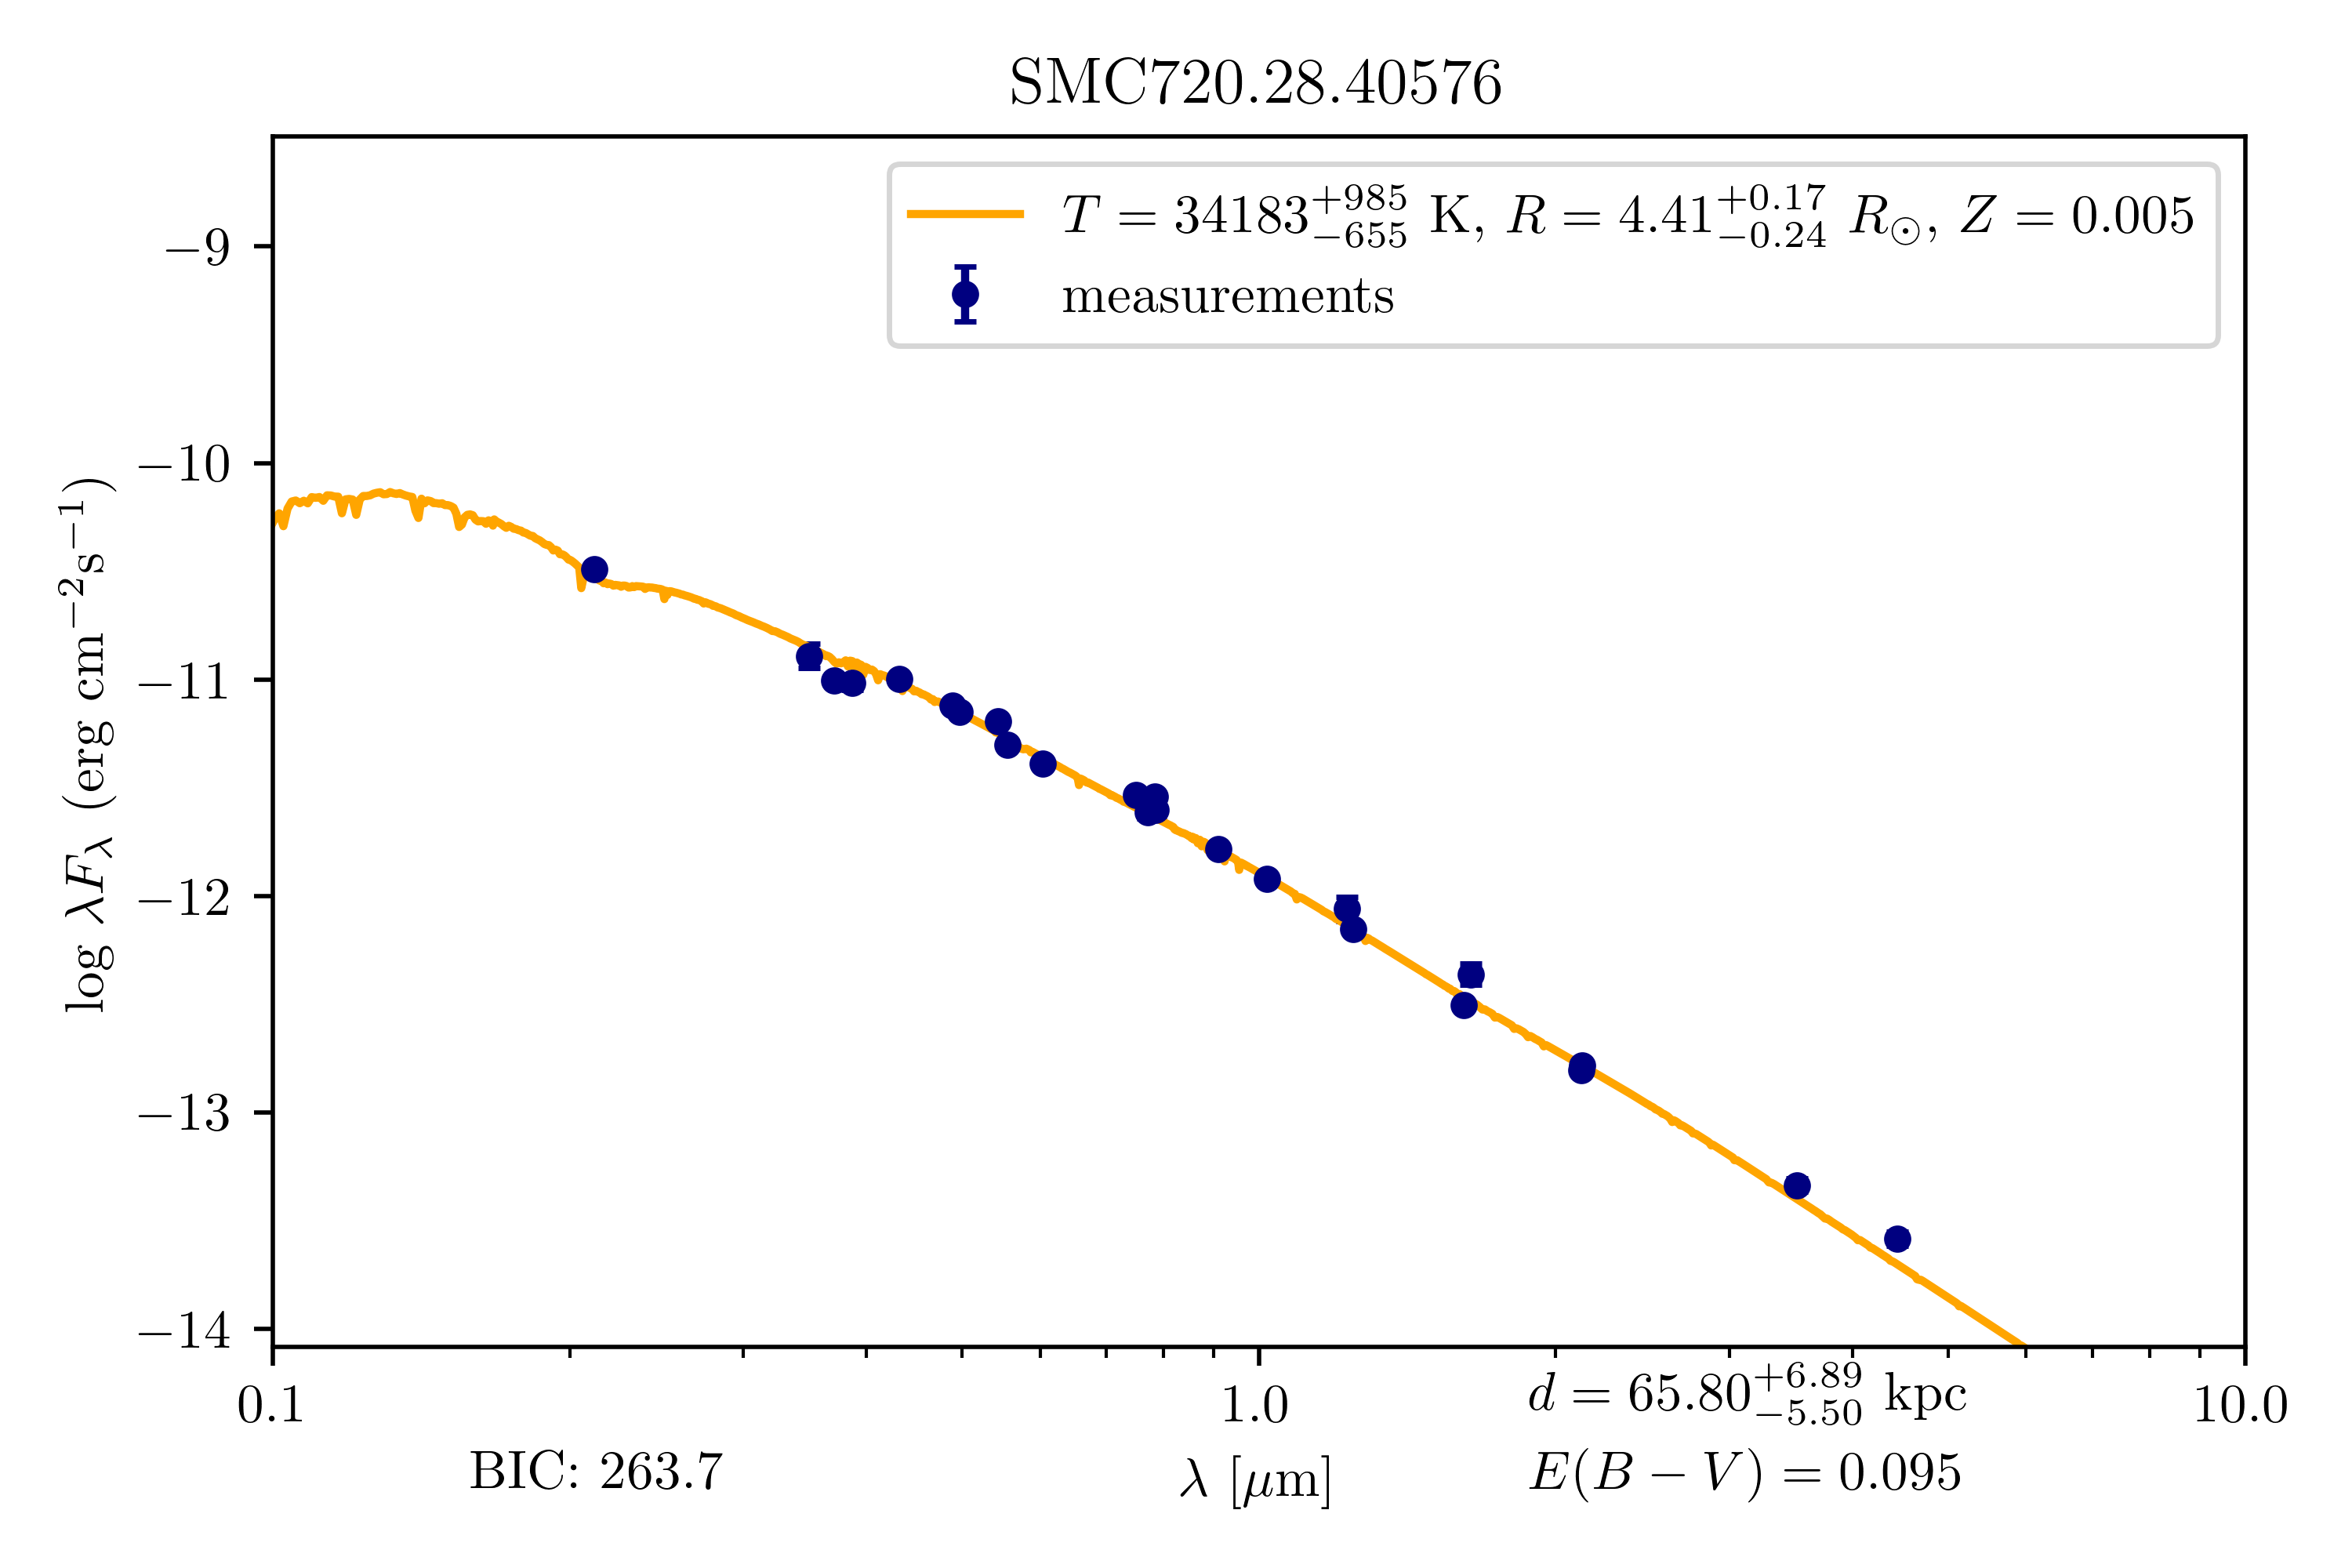
\includegraphics[scale=1]{plots/SMC720.28.40576_simple_emcee.png}
    \caption{Single model SED fit for SMC720.28.40576.}
    \label{SMC720:sed}
\end{figure}
Available data paired with MCMC allow to put some constrains on the parameters of objects even if chain had not converged. 
When MCMC chain isn't able to determine significance of some parameters it's reconstructing prior distribution 
which results in uniformly distributed region of samples. Second MCMC run was performed and $64000$ samples were drown from 
posterior distribution. 
As primary star is supergiant second SED fit is performed assuming $\log g_1=4$ and $\log g_2=4$ as one expect secondary component to be 
main sequence star. 
Results of MCMC sampling were plotted over samples from HYG
database\footnote{https://www.astronexus.com/hyg} and are presented on figure \ref{posterior}
\begin{figure}[H]
    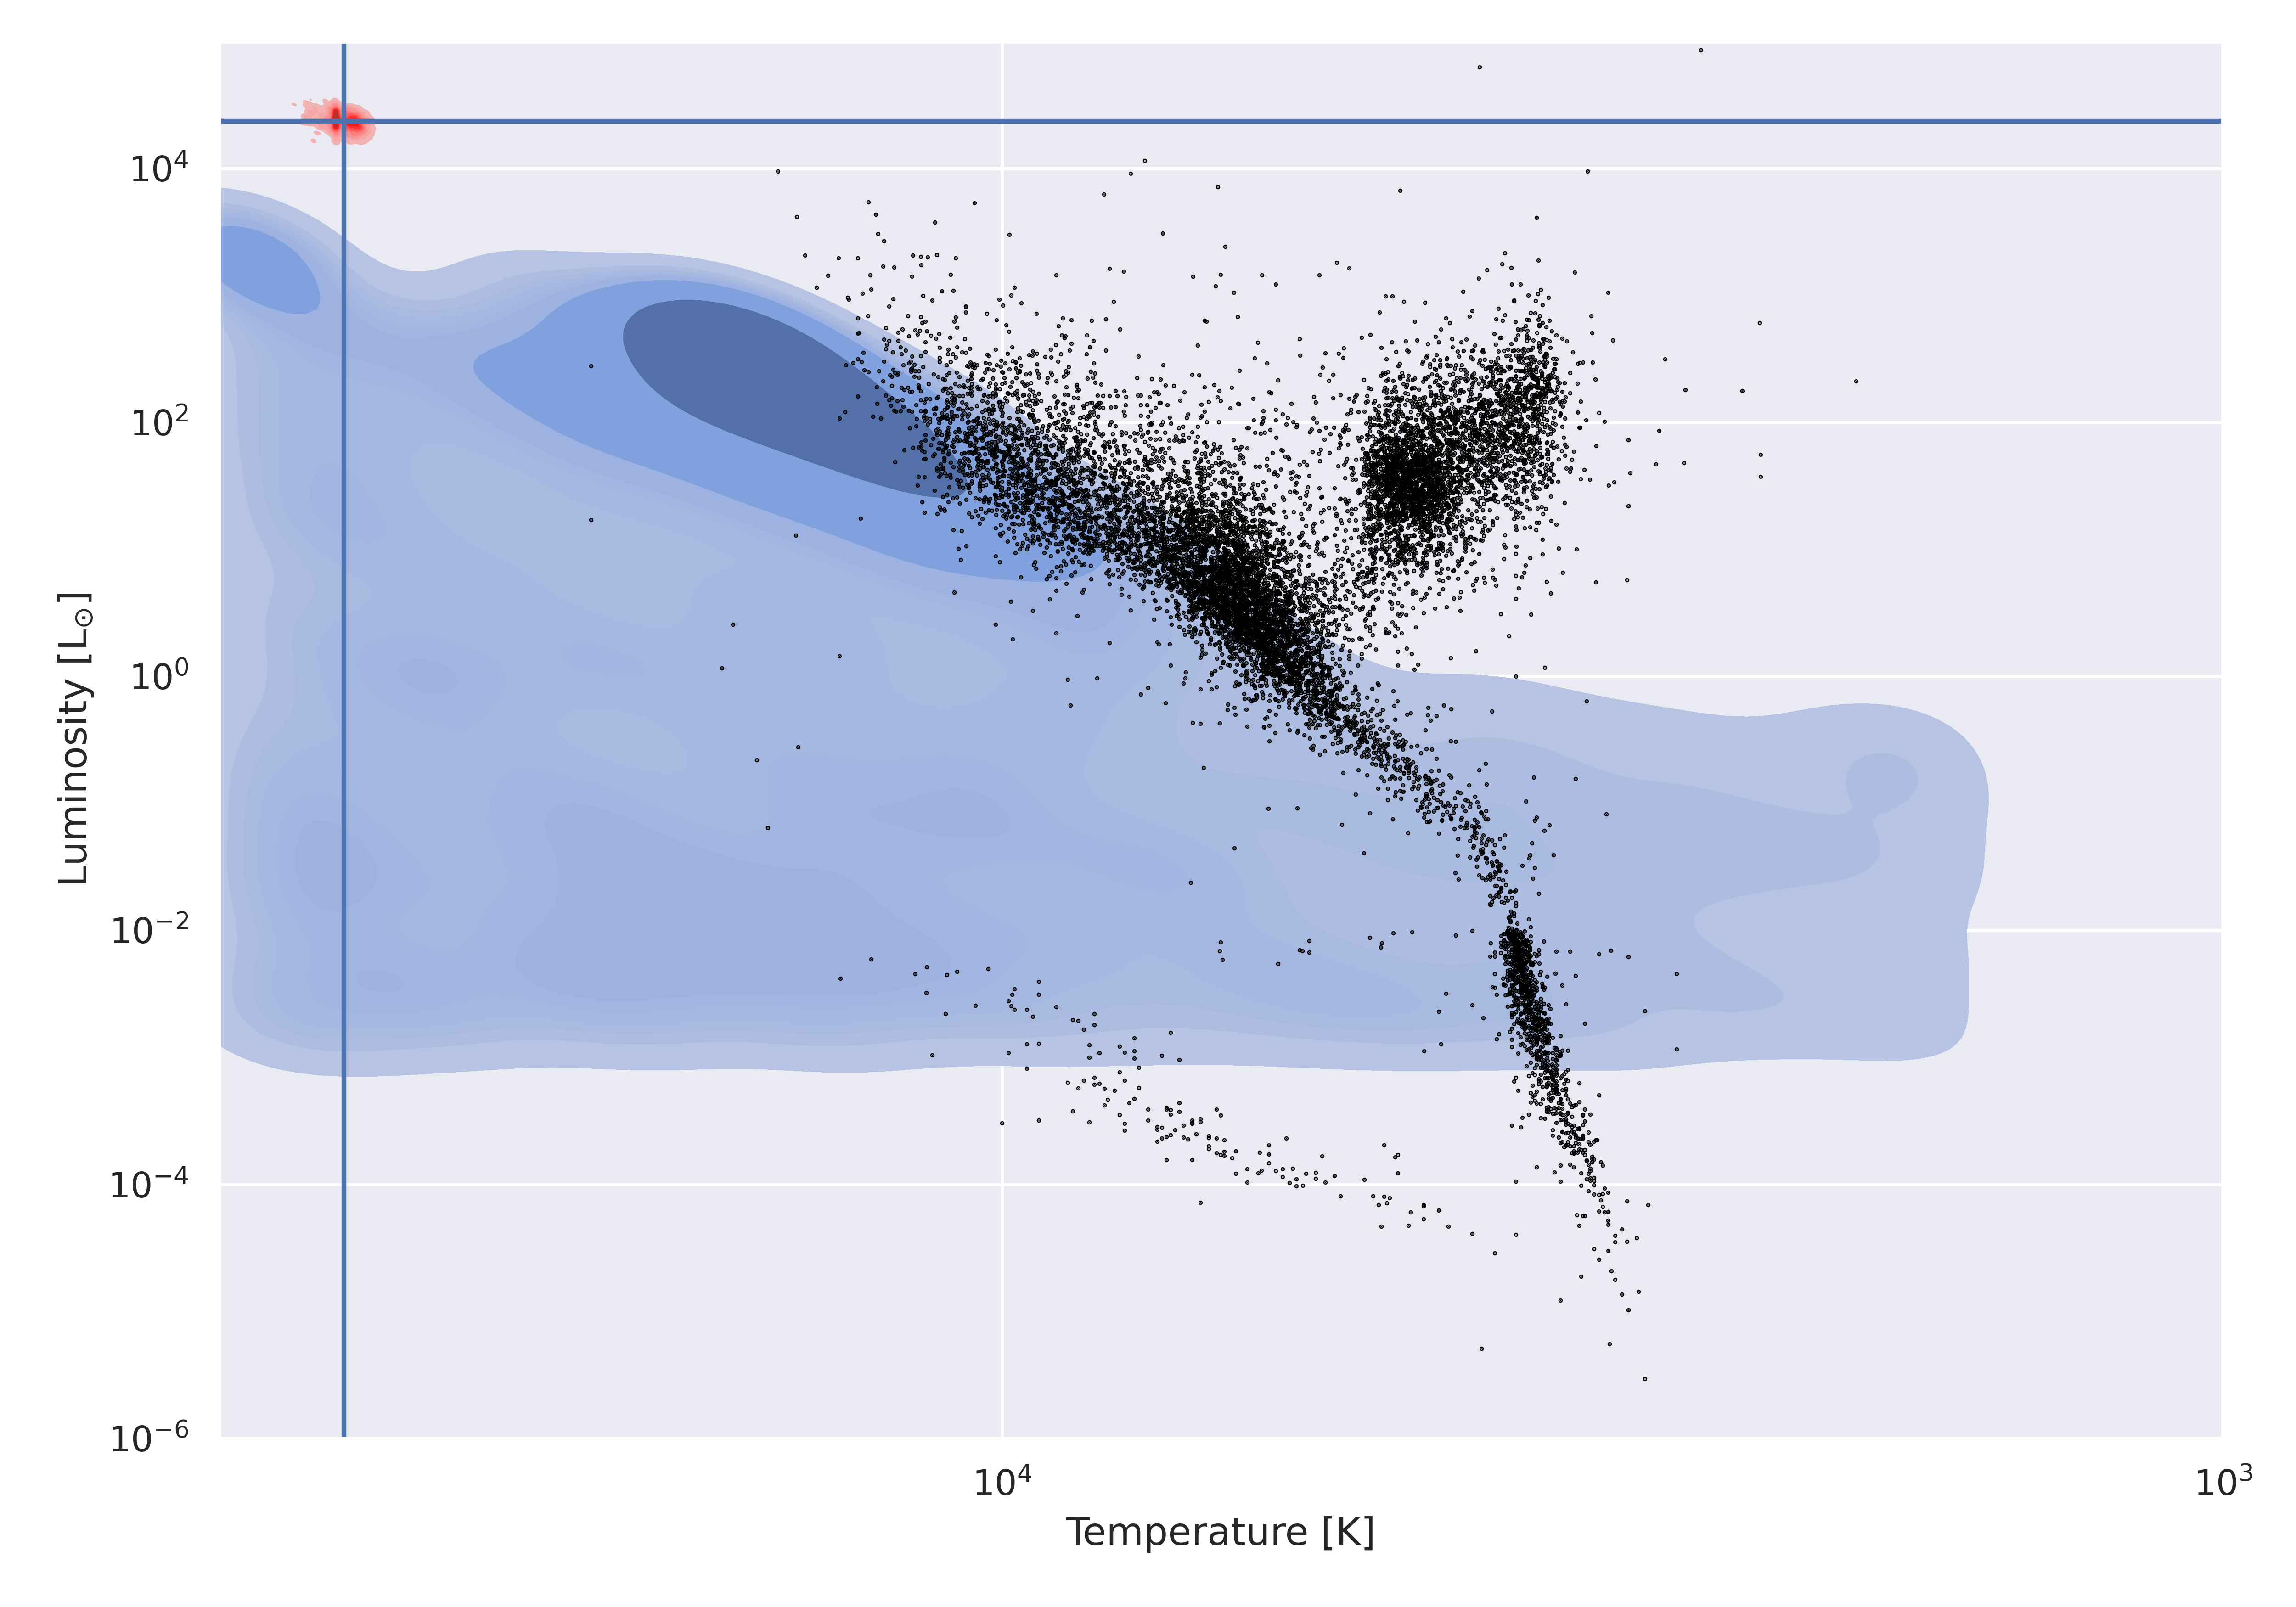
\includegraphics[scale=0.6]{plots/posterior_estimate_SMC720.png}
    \caption{Posterior estimate for parameters of SMC720.28.40576 highlighted in red (primary component)
    and in blue (secondary component).}\label{posterior}
\end{figure}
We can see, that samples fill the space almost uniformly but omit region populated with cold and luminous stars as 
those are to luminous in infrared to reproduce observed values.
Although we can rule out any objects on giant branch many regions on HR diagram can host potential secondary companion, most importantly
few regions of main sequence stars cannot be ruled out giving plausible candidate for secondary companion.
\subsection{Rest of objects}
Majority of objects on the list can be characterized as objects with intermediate temperature. The typically have radius in order of 
few solar radii and spectral type from G to A. Although no detailed information about objects was found two of them
are listed as non-single stars in Gaia DR3 Eclipsing Binaries catalog (BLG986.08.7, BLG931.27.36745).
Catalog contains stars with collected light curves that matched precomputed set of eclipsing/ellipsoidal binaries. 
Detailed processing steps can be found in Gaia documentation \footnote[1]{https://gea.esac.esa.int/archive/documentation/GDR3/Data\_analysis/chap\_cu4nss/sec\_cu4nss\_eclipsing\_bin/}
. After matching the light curve with precomputed set best model serves as start in local optimiser 
trying to further refine solution. Model is solved with respect to parameters:
\begin{itemize}
    \item fillout factors of stars $s_1$, $s_2$.
    \item inclination $i$
    \item temperature ratio $T_1/T_2$ (effective values)
    \item argument of periastron $\omega$
    \item time $t_0$ of eclipse
\end{itemize}. 
Both objects reported by Gaia DR3 are fitted with contact binary model where $s_1>1$ and $s_2>1$ with almost no 
temperature difference (ratio close to $1$). This results pointed out that it's possible to obtain similar results 
in the contact system with same temperature for both stars fooling SED fit. 
This line was further investigated and each object was fitted using 
PHOEBE simulation software (\citet*{wilson_realization_1971},\citet*{prsa_computational_2005},\citet*{conroy_physics_2020}). Model was constructed in such way that both stars shared temperature $T$ (infered from 
single model SED) and were overflowing their Roche lobes.
While masses of objects were free parameters radii are chooses to retain total luminosity of system $R_1^2+R_2^2=R_{single}^2$ where $R_{single}$ denotes 
fitted value from SED. Two masses together with inclination $i$ form three parameters that are fitted to minimize $\chi^2$ using Nelder-Mead algorithm.
Fitted values together with $\chi^2$ values are presented in the table \ref{light_curve_fits} together with predicted semi-amplitude of velocity together 
with estimated one if available from Gaia DR3 data.
\begin{table}[H]
    \normalsize
    \begin{center}
    \begin{tabular}{lllllll}
    Name & $M_1$ [M$_{\odot}$] & $M_2$ [M$_{\odot}$] & $i$ & $K_{estimate}$ [km/s] & $K_{Gaia}$ [km/s]&$\chi^2/dof$ \\
    BLG931.27.36745 & $0.81$ & $0.20$ & $49.71^\circ$ & $36.23$ & $47.26$ & $828.44/74$ \\
    GD1097.20.2300 & $1.45$ & $0.36$ & $59.98^\circ$ &$57.97$& $75.03$ & $2745.79/118$ \\
    BLG986.08.7 & $1.42$ & $0.36$ & $46.65^\circ$ & $117.52$ & $79.14$ & $777.11/72$ \\
    GD2246.03.1814 & $1.05$ & $0.26$ & $53^\circ$ & $73.28$ & $129.93$ & $1926.87/124$\\
    GD1448.27.17 & $1.54$ & $0.39$ & $48.30^\circ$ & $84.23$ & $40.69$ & $4629.40/184$\\
    \end{tabular}
    \caption{Table with parameters used to fit light curves of objects together with radial velocities estimates and 
    normalized $\chi^2$ values.}
    \end{center}
    
    \caption{Estimated mass function using Gaia radial velocity error.}\label{light_curve_fits}
\end{table}
One example light curve fit for object BLG931.27.36745 can be seen on the plot \ref{lc_plot}.
One could ask how presented fits compare to the theory introduced at the beginning where it was theoretized that 
such objects should have mass ratio $q>1$. Theory presented in \citep{gomel_search_2021} together with PHOEBE simulations treated only semi-detached case
so modified mass ratio is strictly limited to those types of objects. Although there is no guarantee that presented models
describe actual parameters of binaries there are good alternative for compact companions. Contrary to compact objects 
which are quite uncommon presented contact binaries are much more numerous.
\begin{figure}
    \begin{center}
        \includegraphics[scale=0.7]{plots/modeling_phoebe_contact_BLG931.27.36745.jpg}
    \end{center}
    \caption{Light curve fit with contact binary for BLG931.27.36745 calculated using PHOEBE.}\label{lc_plot}
\end{figure}

\chapter{Discussion}
Out of total $8515$ objects investigated in this study only $14$ objects were classified as plausible candidates for binaries with compact companions.
Further investigation into sample revealed one rotational variable and suggested alternative explanation for $12$ objects in the form of
contact binaries with intermediate mass ratio. For $7$ objects mass function was calculated and revealed no interesting objects as for most of them 
$f(m_1,m_2,i)<0.1$ M$_{\odot}$. Only object with higher mass function is GD1070.18.22288 which is likely rotational variable with unknown orbital period 
resulting in useless mass function. It's hard to determine what is accuracy of mass function estimation  which can be skewed by many factors.
Those doubts begin to strengthen if we assume that objects are composed of two stars with similar temperature as suggested by light curve analysis.
In this case it's unknown what to expect as spectra of objects are composed of two base objects which can be hard to process by Gaia pipeline.
Up to date only one work \citep{nagarajan_spectroscopic_2023} tries to perform any kind of follow-up observations of 
candidate BH binaries reported in \citep{gomel_gaia_2022} which were identified using method presented in \citep{gomel_search_2021}. 
This publication is one step ahead with respect to this work as spectroscopic follow-up was performed allowing to estimate amplitude of velocity 
with much higher precision then very crude estimation based on Gaia DR3 radial velocity measurements. Nevertheless presented results match those 
presented in the work as most of the objects share many physical parameters. It was pointed out that 
method used to identify objects is based on the assumption that objects nearly fill their Roche Lobes what occurs during relatively
short period of binaries lifetime. Contact binaries although rare outcome of evolution are expected to be quite common compared to any kind of compact 
objects. Light curve modeling with contact binaries isn't able to explain all of variability so fit might need some refining but even if 
contact model fails in some cases it's still provides quite good explanation for observed variability. Most importantly estimated amplitude of such 
modulation can easily reach values set at threshold for which $q_{mmr}>1$ resulting in huge number of false positives.
Although no final conclusion is reached results seem to support conclusion of \citep{nagarajan_spectroscopic_2023}. In order to further 
characterize objects more observations should be conducted.


\bibliography{Bachelor} 
\bibliographystyle{mnras}
\begin{appendices}
    \chapter{Semi-amplitude estimate from Gaia DR3}
    Let's now assume, that this radial velocity can be factored into two separate movements: center of mass movement (with velocity $v_0$) and circular motion with semi-amplitude $K$. Under following 
assumptions we can find, that samples of radial velocity can be written as 
\begin{equation}
    V_i=v_0+K\cos{(2\pi X_i)}
\end{equation}
where $X_i$ is sample from $\mathcal{U}(0,1)$. This allows to determine, that if we write down our statistics of $\sigma^2$ we get 
\begin{equation}
    \sigma^2=\frac{1}{n}\sum_i (\overline{V}-V_i)^2\approx \frac{K^2}{N}\sum \cos^2{(2\pi X_i)}=\frac{K^2}{N}\sum_i \frac{\cos{(4\pi X_i)}+1}{2}
\end{equation}
where we used the simplification that $\overline{V}\approx v_0$. Now we would like to obtain some statistical properties of this variance estimator such as expected value and variance.
We can clearly see that $\mathbb{E}\cos{(4\pi X_i)}=0$ while $\Var(\cos{4\pi X_i})=\frac{1}{8}$. While first value is straightforward as mean of cosine is equal to zero second one 
is more complicated but follows from the fact that $\cos{(4\pi X_i)}$ is arcsine distributed and it's variance it's well known. Hence we see, that 
\begin{align}\label{semi}
    \mathbb{E} \sigma^2 = \frac{K^2}{2N}\cdot N = \frac{K^2}{2}\\ 
    \Var (\sigma^2) = \frac{K^4}{32N^2}\cdot N = \frac{K^4}{32N}
\end{align} 
Those two values allow us to determine quality of our estimator, using Central Limit Theory one can also approximate that 
\begin{equation}
    \sigma^2 \sim \mathcal{N}\left(\frac{K^2}{2},\frac{K^4}{32N}\right)
\end{equation}
which can be quite useful to estimate $K$ from obtained data (for most of the objects $N>17$ so Central Limit Theorem gives good approximation).
There are many simplification made here which are mainly based on the fact it's not entirely know how Gaia obtains RV measurements and what is measured after all.
If we assume, that true velocity is contaminated by gaussian noise with standard deviation $\sigma_{noise}$ estimated variance will be shifted and 
\begin{equation}
    \mathbb{E} \sigma^2 = \frac{K^2}{2}+\sigma_{noise}^2
\end{equation} 
so we will overestimate $K$.
    \end{appendices}
\end{document}